\documentclass[11pt,a4paper]{article}

\usepackage{geometry}
\geometry{margin=2.5cm}
\usepackage{graphicx}
\usepackage{booktabs}
\usepackage{amsmath}
\usepackage{amssymb}
\usepackage{xcolor}
\usepackage[numbers,sort&compress]{natbib}
\usepackage{hyperref}
\hypersetup{hidelinks}
\setlength{\textfloatsep}{8pt plus 2pt minus 2pt}
\setlength{\floatsep}{8pt plus 2pt minus 2pt}
\setlength{\intextsep}{8pt plus 2pt minus 2pt}
\setlength{\abovecaptionskip}{4pt}
\setlength{\belowcaptionskip}{2pt}
\setlength{\abovedisplayskip}{6pt plus 2pt minus 2pt}
\setlength{\belowdisplayskip}{6pt plus 2pt minus 2pt}

\newcommand{\todo}[1]{\textcolor{red}{[TODO: #1]}}
\makeatletter
\let\paper@thebibliography\thebibliography
\renewcommand{\thebibliography}[1]{%
  \paper@thebibliography{#1}%
  \raggedright
}
\makeatother

\title{Geometric validity is not perceptual quality: what deterministic probes can and cannot measure in generated 3D assets}
\author{Miles Carter\\
modelfy.art (\url{https://modelfy.art})\\
\texttt{support@modelfy.art}}
\date{}

\begin{document}
\maketitle

\begin{abstract}
Geometric validity and perceived quality are different properties of a generated mesh.
We measured how far deterministic, CPU-only mesh probes (boundaries, components, self-intersection, hidden surface, thin walls, roughness) track each, using expert defect labels, human geometry ratings, MLLM pseudo-labels and defects injected into real scans, in pre-registered analyses.
Injected holes and floaters were detected perfectly (AUROC 1.000); interpenetrating parts and crossing sheets at 0.940--0.986, hidden shells at 0.811--0.912, thin fins at 0.952 (two larger severities) and vertex noise at 0.753--0.999, although the hidden-surface and self-intersection checks also respond to other defects.
On 3D-DefectBench expert-agreement cells, a logistic regression on 30 probe features trained only on crowd labels reached a Matthews correlation of 0.272 averaged over three primary geometry defects, against 0.335--0.341 for the best vision-language judges; no paired McNemar test against the four strongest judges was significant, although one bootstrap interval favoured Gemini 3.1 Pro, and form/surface performance was largely explained by generator identity.
Assets that crowd workers judged defect-free were geometrically dirty, while strict checks fired on undamaged scans.
Within generators, correlations with MATE-3D human geometry ratings had absolute value at most 0.2; on 2{,}797 Hi3DBench meshes, correlations with an MLLM Geometry Plausibility score were at most 0.111 in absolute value, did not survive adjustment for prompt, and reversed for a geometric-detail score.
A training-free conjunction of vision-language votes and probe flags raised Matthews correlation in 29 of 36 pairs but was significant in only one.
Such probes are useful validity gates and confound checks, not perceptual judges.
\end{abstract}
\noindent\textbf{Keywords:} 3D generation; mesh quality; geometric validity; vision-language models; defect detection.
% src: results/macro_mcc.csv; results/RESULTS_milestone1.md; results/RESULTS_milestone2.md; results/RESULTS_milestone3.md; results/gso/gso_detection.csv

\section*{Highlights}
\begin{itemize}
  \item Deterministic probes detected injected holes and floaters with AUROC 1.000, and detected self-intersection, hidden shells, thin walls and noise at moderate severity on real scans.
  \item On expert labels the probe is mid-pack among 12 vision-language models and two controls (macro MCC 0.158 over five geometry defects, rank 8 of 15).
  \item Assets that crowd workers called defect-free are geometrically dirty, and clean decimated scans already trip strict validity checks.
  \item Within-generator associations are small for human geometry ratings (absolute Spearman correlation at most 0.2) and smaller for Hi3DBench MLLM pseudo-labels (at most 0.111). The geometric-detail score reverses the sign.
  \item A training-free conjunction with vision-language votes is directionally consistent and, after correction, significant in 1 of 36 comparisons.
\end{itemize}
% src: results/RESULTS_milestone1.md; results/RESULTS_milestone2.md; results/RESULTS_milestone3.md; results/macro_mcc.csv; results/gso/gso_detection.csv

\section{Introduction}
\label{sec:intro}

Text-to-3D and image-to-3D generators now produce meshes that are scored, in most recent benchmarks, by people or by vision-language models (VLMs) looking at renders \citep{poole2022dreamfusion,lin2023magic3d,wu2024gpteval3d,zhang2025mate3d,zhao2026defectbench,zhang2025hi3deval}.
Those judgements answer a perceptual question: does the asset look complete, coherent and faithful to the prompt?
A second question is geometric.
Does the mesh contain holes, disconnected fragments, self-intersections, internal shells or walls thinner than a stated tolerance?
Graphics has long treated that second question as a repair and printability problem \citep{attene2010meshfix,zhou2016thingi10k,garland1997qem}.
Fabrication studies of generative meshes still record defects by hand and leave automatic detection as future work \citep{faruqi2026instructmesh}.

The two questions are easy to conflate, because several benchmarks describe perceptual failures with geometric words (``fused'', ``incomplete'', ``extra geometry'', ``bad surface'').
3D-DefectBench makes the conflation testable.
It releases meshes, expert and crowd labels for fine-grained defects, and the predictions of 12 VLMs, and it does not include a mesh-geometric baseline \citep{zhao2026defectbench}.
We used that release, together with human geometry ratings from MATE-3D \citep{zhang2025mate3d} and synthetic defects injected into Google Scanned Objects (GSO) scans \citep{downs2022gso}, to measure what a frozen family of deterministic probes can and cannot see.

The working distinction, which the measurements support, is between \emph{geometric validity} and \emph{perceived quality}.
Validity here means a pre-declared, scale-normalised property of the triangle mesh: boundary length, component structure, self-intersection, hidden surface, local thickness, or dihedral roughness.
Perceived quality means an expert vote, a crowd vote, or a human geometry rating.
A valid mesh can still look wrong, and a mesh that raters call clean can still fail a strict geometric check.
The probes are cheap, deterministic and fully specified.
They are complements to perceptual and VLM judges, useful as validity gates and as a way to expose generator confounds.
On the expert cells they are comparable to mid-tier VLM judges, and they do not replace the strongest ones.

\paragraph{Contributions.}
\begin{enumerate}
  \item A documented CPU-only probe suite (Section~\ref{sec:method}) and a pre-registered comparison with the 12 VLM judges released by 3D-DefectBench, plus a face-count control and a generator-identity control.
  We did not query any VLM.
  \item An external check on MATE-3D human geometry ratings that separates pooled, within-generator, within-prompt and two-way fixed-effect estimands, so that a generator confound is visible rather than absorbed into a single correlation.
  \item A controlled injection study on 120 GSO scans that reports detection, cross-talk, and the gap between a strict zero threshold and a threshold calibrated on generated assets that crowd workers called defect-free.
  \item Family ablations and both a training-free and a learned fusion with VLM votes, including the negative and null results: the form/surface association is largely a generator effect, topology-only performance on the expert cells is a test-set observation, and the conjunction rule is directionally consistent but rarely significant after correction.
  \item A pre-registered secondary analysis of Hi3DBench (Section~\ref{sec:hi3d}).
  The scores are MLLM pseudo-labels from the Hi3DEval multi-agent pipeline, not human ratings \citep{zhang2025hi3deval}.
  Within-generator correlations with Geometry Plausibility meet the pre-registered sign but are small (absolute value at most 0.111), are not robust to prompt adjustment, and reverse for a geometric-detail score.
  Agreement with that automated judge is not human validation.
  % src: results/RESULTS_milestone3.md; results/hi3dbench/hi3dbench_correlations.csv
\end{enumerate}

\section{Related work}
\label{sec:related}

\subsection{Perceptual and VLM evaluation}
Text-to-3D methods were first compared largely by inspection of renders \citep{poole2022dreamfusion,lin2023magic3d,wang2023sjc,metzer2022latentnerf,tsalicoglou2023textmesh}.
Later benchmarks make that inspection repeatable.
T$^3$Bench scores alignment and quality from multi-view renders \citep{he2023t3bench}.
GPTEval3D showed that a VLM can track human rankings \citep{wu2024gpteval3d}.
Eval3D argues for fine-grained criteria rather than one score \citep{duggal2025eval3d}, and Gen3DEval uses vision-language models as automatic judges \citep{maiti2025gen3deval}.
MATE-3D collects multi-dimensional human ratings, including a geometry mean opinion score, on 1{,}280 meshes from eight generators \citep{zhang2025mate3d}.
% src: results/mate3d/mate3d_dec10k_meta.json
A later benchmark follows the same perceptual direction at finer granularity \citep{cui2025fine}.
3DGen-Bench releases human preferences over a broad generator set; we did not use it, because the data files are gated \citep{zhang2025gen3dbench}.

3D-DefectBench changes the unit from a scalar preference to binary, fine-grained defects, and it varies the VLM pipeline \citep{zhao2026defectbench}.
The release contains expert labels, a crowd-labelled silver holdout, meshes and predictions from 12 VLMs.
Those VLMs are compared with a CLIP zero-shot baseline \citep{radford2021clip}.
The paper does not evaluate a non-learned mesh baseline.
% src: results/macro_mcc.csv
DB-3DME studies human-aligned automatic mesh scores \citep{jia2026db3dme}.
The release we inspected provides GIF renders rather than meshes, under the MIT licence on the dataset card, so the probes could not be run.
Hi3DEval proposes a hierarchy of validity, geometry and texture scores \citep{zhang2025hi3deval}.
Its published object-level scores are produced by an automated MLLM pipeline.
We treat them as pseudo-labels.

\subsection{Geometric metrics, repair and fabrication}
When a target surface exists, Chamfer distance, IoU and F-score are the usual scores, and the choice among them changes the conclusion \citep{tatarchenko2019single}.
The benchmarks above do not provide a unique target surface.
Perceptual metrics trained on distortions of artist or scanned meshes address a different question again \citep{nehme2023tmqa}.
Repair tools already name several validity failures: MeshFix for some topological and geometric defects of digitised solids \citep{attene2010meshfix}, quadric simplification for a face budget \citep{garland1997qem}, and MeshLab for both simplification and a per-face self-intersection test \citep{cignoni2008meshlab}.
Thingi10K showed how common such defects are in models people try to print \citep{zhou2016thingi10k}.
InstructMesh classified fabrication defects on reconstructions from a single generator by hand, and left automatic detection open \citep{faruqi2026instructmesh}.
We use that vocabulary as a fixed function of every face, and we compare the decisions with human labels and VLM votes on the same assets.
Implementation uses Trimesh and Embree \citep{trimesh,wald2014embree}.

\subsection{What is compared here}
Perceptual benchmarks answer preference, prompt alignment and texture.
They do not say whether a ``defect-free'' vote implies a mesh without holes, floaters, self-intersections, internal shells or thin walls, or whether a failure a probe can name is the failure a rater named.
That comparison was pre-registered.
MCC is used because accuracy is misleading under imbalance \citep{chicco2020mcc}, paired decisions use McNemar's test \citep{mcnemar1947}, multiplicity uses the Benjamini--Hochberg procedure \citep{benjamini1995fdr}, and intervals are percentile bootstraps \citep{efron1993bootstrap}.
The design choice is to apply these separately to validity and to perception, with a generator-only baseline in every human-label analysis.

\section{Probes}
\label{sec:method}

\subsection{Normalisation}
Every probe reads a triangle mesh after a deterministic normalisation.
The bounding box is centred at the origin and scaled so that its diagonal equals 1.
Vertices are then welded by rounding coordinates to \(10^{-6}\) and replacing each welded group by its mean.
All lengths reported below are therefore in units of the bounding-box diagonal, and the probes have no learned parameters.
Area-weighted samples use a fixed random seed, so a given file and library build produce the same scalars.
Configuration constants are collected in Appendix~\ref{app:probes}.
% src: geomcheck/probes.py

When a mesh has more than 10{,}000 faces we optionally decimate it, before probing, to 10{,}000 faces by quadric edge collapse with topology, boundary and normal preservation and planar quadrics enabled \citep{garland1997qem,cignoni2008meshlab}.
3D-DefectBench meshes already lie at or below about 10.7k faces (median 8{,}119), which is the regime in which the classifier was trained, so the expert-set evaluation does not decimate.
MATE-3D and the GSO injection study do.
A faster decimator was rejected before any scoring because it opened holes; that deviation is recorded in Appendix~\ref{app:prereg}.
% src: results/RESULTS_milestone1.md; results/runtime_summary.csv; geomcheck/probes.py; analysis/PREREGISTRATION_M2.md

\subsection{Feature families}
We compute eight feature families (size, boundary/manifold, topology, triangle quality, roughness, self-intersection, hidden surface and thin wall), described in six groups below.
Unless noted, fractions are over faces, edges or samples as stated.

\paragraph{Size and boundary.}
Face count; fraction of duplicate faces; fraction and total length of boundary edges; number of boundary loops; fraction of two-manifold edges whose two directed half-edges fail to cancel (winding); fraction of non-manifold edges.
A mesh is recorded as watertight when it has no boundary and no non-manifold edge.

\paragraph{Topology.}
Face-adjacency components, the area fraction of the largest component, the number and area fraction of components smaller than 1\% of the surface, and the number of remaining components.
The genus proxy is
\begin{equation}
g = \max\bigl(0,\, 2C - \chi\bigr) / 2,
\label{eq:genus}
\end{equation}
where \(C\) is the number of components and \(\chi = V - E + F\), with \(V\) the number of vertices referenced by a face.
The classifier receives \(\log(1+g)\).

\paragraph{Triangle quality.}
For a triangle of area \(A\) and edge lengths \(a,b,c\),
\(q = 4\sqrt{3}\, A / (a^2+b^2+c^2)\), which equals 1 for an equilateral triangle and 0 for a degenerate one.
We store the median and the 5th percentile of \(q\), the fraction of faces and of area with \(q < 0.1\) (slivers), and the coefficient of variation of edge length.

\paragraph{Roughness.}
On each interior manifold edge we take the angle between the two incident face normals.
We store the length-weighted mean angle in degrees and the length fraction above \(30^\circ\), \(60^\circ\) and \(90^\circ\), plus the mean and 95th percentile of absolute angle defect on interior manifold vertices.

\paragraph{Self-intersection.}
PyMeshLab marks faces that intersect another face of the same mesh \citep{cignoni2008meshlab}.
We store the fraction of faces and of area that are marked.

\paragraph{Hidden surface and thin walls.}
We draw 20{,}000 area-weighted points on the surface.
A point is hidden when a ray from it fails to escape in every one of 64 Fibonacci directions (Embree) \citep{wald2014embree}.
Thickness at a point is the length of the shorter ray along the outward or inward normal that exits through a face whose normal agrees with the ray.
We store the fraction of samples at which thickness is defined, the median thickness, and the fraction of samples thinner than \(0.005\) and \(0.010\) diagonals.
% src: geomcheck/probes.py

Features with zero variance on the training split were dropped.
The classifier uses the remaining 30 features.
Figure~\ref{fig:pipeline} shows the path from a file to those features and to the frozen scores.

\begin{figure}[t]
  \centering
  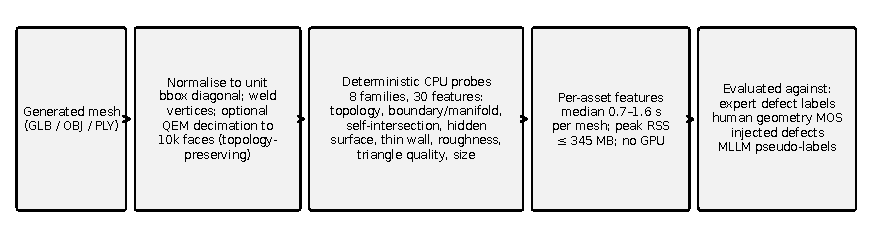
\includegraphics[width=\linewidth]{figures/fig1a_pipeline.pdf}
  \caption{Probe pipeline. A mesh is normalised to a unit bounding-box diagonal, welded, and, outside 3D-DefectBench, decimated to 10{,}000 faces. Deterministic features are then passed to a logistic regression whose weights and thresholds were frozen on the silver holdout.}
  \label{fig:pipeline}
\end{figure}

\subsection{Frozen classifier and controls}
The primary predictor, GeomProbe-LR, is one L2 logistic regression per defect.
Features are transformed by \(\log(1+x)\) (genus as above) and standardised with the mean and variance of the training split.
The regression uses \(C = 1\), balanced class weights and at most 5{,}000 iterations.
The decision threshold maximises Matthews correlation coefficient (MCC) on the five-fold stratified out-of-fold probabilities of the training split (shuffle, seed 0).
The model is then refit on the whole training split.
Nothing---features, \(C\), or thresholds---was chosen on the expert set.
% src: analysis/PREREGISTRATION.md

Two controls use the same threshold rule.
FaceCount-LR sees only \(\log(1+n_{\text{faces}})\).
Generator-only sees only the generator identity.
For 3D-DefectBench that identity is the benchmark's model A or model B.
We also report the within-generator AUROC of GeomProbe-LR so that a between-generator difference is not mistaken for a geometric effect.

VLM comparisons use the binary votes released with 3D-DefectBench (configuration c004, successfully parsed rows only) \citep{zhao2026defectbench}.
For a binary vote, AUROC equals balanced accuracy; we label it as such.
Probe AUROC uses the predicted probability.
MCC and F1 are computed for every predictor.
Our macro-MCC values for the 12 VLMs reproduce those reported by the benchmark authors to three decimal places; the match was checked before the expert-set plan was written, as a label-handling test, and it is not a result about geometry.
% src: analysis/PREREGISTRATION.md; results/RESULTS_milestone1.md

\subsection{Injection operators}
On each cleaned GSO mesh we apply seven operators at three severities (S1 \(<\) S2 \(<\) S3), using a per-object seed.
Holes delete three surface patches whose total area is 0.2\%, 1\% or 4\% of the mesh.
Floaters add 1, 3 or 10 icospheres of radius 0.01, centred 0.05 off the surface along the normal.
An interpenetrating part is an ellipsoid of major radius 0.05, 0.10 or 0.20, concatenated without a Boolean union.
A thin fin is a \(0.2 \times 0.2\) plate of thickness 0.008, 0.004 or 0.002, half-embedded at a surface point.
Noise displaces vertices along their normals by a Gaussian of standard deviation 0.001, 0.003 or 0.01.
A crossing sheet duplicates a patch of area 0.5\%, 2\% or 5\% and rotates the copy by \(30^\circ\).
A hidden shell places an icosphere, of radius 0.25, 0.50 or 0.90 times the distance from an interior point to the surface, at the point farthest from the surface among 20{,}000 uniformly sampled interior candidates.
Objects with no interior point would have been skipped and counted; none were.
% src: scripts/gso_inject.py; analysis/PREREGISTRATION_M2.md; results/RESULTS_milestone2.md

Each operator has a pre-registered target check.
Holes map to boundary-edge fraction, and floaters to the small-component count.
Interpenetration maps to self-intersection and also to hidden surface.
Fins map to the thin-wall fraction at 0.005, and noise to the length-weighted dihedral mean.
Crossing sheets map to self-intersection, and internal shells to hidden surface.
S1 fins are thicker than 0.005 by design.
The 0.010 thin-wall check is the one expected to see them.
% src: analysis/PREREGISTRATION_M2.md; results/RESULTS_milestone2.md

\section{Data and protocol}
\label{sec:data}

\subsection{Datasets and licences}
Table~\ref{tab:datasets} lists the four corpora that were scored, their licences, and the cost of probing them.
All runs were CPU-only, on an 8-core machine with about 6\,GB of usable memory and no GPU.
Times are median and 95th percentile wall-clock seconds per mesh with four parallel workers, and they include decimation where it was applied.

\begin{table}[t]
  \centering
  \caption{Datasets scored in this study. ``Probed OK'' counts meshes that returned a full feature vector. Peak RSS is the resident set of one worker. Runtimes use four parallel workers on an 8-core CPU and include decimation for MATE-3D and Hi3DBench. Hi3DBench contributes 3{,}060 probed meshes, of which 2{,}797 labelled meshes are analysed. Its labels are MLLM pseudo-labels.}
  \label{tab:datasets}
  \begingroup
  \makeatletter
  \let\paper@arrayparboxrestore\@arrayparboxrestore
  \def\@arrayparboxrestore{\paper@arrayparboxrestore\raggedright}
  \makeatother
  \resizebox{\linewidth}{!}{% generated by paper/scripts/fig_results.py from results/runtime_summary.csv
\begin{tabular}{p{3.2cm}rrp{3.0cm}p{3.4cm}rrr}
\toprule
Dataset & Meshes & Probed OK & Labels & Licence & Time/mesh (s) med [P95] & Peak RSS (MB) med [max] & Faces (med.)\\
\midrule
3D-DefectBench (expert + silver) & 678 & 678 & expert + crowd defect labels & CC BY-NC 4.0 (non-commercial research use; no redistribution of GLBs) & 0.67 [0.84] & 158 [163] & 8,119\\
MATE-3D & 1,280 & 1,280 & human MOS (geometry) & CC BY 4.0 & 1.61 [3.20] & 181 [258] & 10,000\\
GSO + injected defects & 2,640 & 2,640 & known injected defect & CC BY 4.0 (scans); injections ours & 0.90 [1.53] & 164 [170] & 9,520\\
Hi3DBench (secondary) & 3,060 & 3,060 & MLLM pseudo-labels (geometry plausibility); 2,797 labelled meshes analysed & MIT (HF dataset card) & 1.36 [3.02] & 182 [345] & 10,000\\
\bottomrule
\end{tabular}
}
  \endgroup
\end{table}
% src: tables/tab_datasets.tex; results/runtime_summary.csv

3D-DefectBench is released under CC BY-NC 4.0 \citep{zhao2026defectbench}.
We used it for non-commercial research.
The GLBs are not redistributed; the release accompanying this paper is code and per-asset probe statistics.
The expert split has 129 assets labelled by two experts.
The silver holdout has 549 assets with crowd majority-vote labels.
One silver asset (identifier 609) is byte-identical to an expert asset and was excluded from every training and threshold fit, leaving 548 training assets.
The primary test cells are those on which both experts agreed.
That is the set for which the benchmark releases VLM predictions: 101 assets for fused/incomplete (17 positive), 88 for form/surface (51 positive) and 121 for extra geometry (6 positive).
Missing parts (12 positives out of 104) and pose/placement (2 positives out of 125) are pre-registered negative controls, because a prompt-blind geometric probe has no access to the text that defines those failures.
Texture defects were not scored.
A secondary probe-only target marks an asset positive if either expert did.
% src: analysis/PREREGISTRATION.md; results/main_comparison_expert_agreement.csv; results/RESULTS_milestone1.md

MATE-3D is released under CC BY 4.0 \citep{zhang2025mate3d}.
We used all 1{,}280 meshes: 160 prompts times eight generators (3DTopia, Consistent3D, DreamFusion, Latent-NeRF, Magic3D, One-2-3-45++, SJC and TextMesh) \citep{hong2024threedtopia,wu2024consistent3d,poole2022dreamfusion,metzer2022latentnerf,lin2023magic3d,liu2023one2345pp,wang2023sjc,tsalicoglou2023textmesh}.
The target is the human geometry MOS.
Every mesh probed successfully, both after decimation to 10{,}000 faces and, as a secondary run, on the raw meshes.
% src: results/RESULTS_milestone2.md; results/mate3d/mate3d_dec10k_correlations.csv; results/runtime_summary.csv

GSO scans are released under CC BY 4.0 \citep{downs2022gso}.
We drew a seeded random subset of 120 objects from the Google Research Fuel collection, welded and decimated each scan, and attached the seven injected defects at three severities.
That is 22 variants per object and 2{,}640 meshes, with no probe failures and no skipped shells.
Hi3DBench is released under the MIT licence on its dataset card \citep{zhang2025hi3deval}.
We probed 3{,}060 meshes (510 for each of SPAR3D, TRELLIS, TripoSR, InstantMesh and Hunyuan3D, and 510 for CRM, of which 247 are labelled) with no probe failures, and we analysed the 2{,}797 labelled meshes.
Those object-level scores are MLLM pseudo-labels.
The comparison is secondary evidence, not a human validation (Section~\ref{sec:hi3d}).
% src: results/RESULTS_milestone2.md; results/RESULTS_milestone3.md; results/gso/gso_detection.csv; results/hi3dbench/hi3dbench_meta.json; results/runtime_summary.csv; tables/tab_datasets.tex; analysis/PREREGISTRATION_M3_hi3dbench.md

\subsection{Pre-registration}
The 3D-DefectBench analysis was committed before any expert-set score was computed (commit 024f7eb, 2026-09-27 16:22 UTC+8).
The MATE-3D, GSO and ablation analysis was committed before those scores were computed (commit 78d6623, 16:44 UTC+8).
The Hi3DBench plan was committed before those meshes were scored (commit c003104, 17:36 UTC+8).
The analysis script was committed as b528343, also before scoring.
The plans themselves state what had already been looked at: VLM files, used only to confirm that our MCC implementation matches the benchmark to three decimals; label counts; an engineering smoke test; and, for decimation, eight meshes of one MATE-3D prompt.
No probe--label correlation entered the plans.
Deviations are listed in Appendix~\ref{app:prereg}.
Thresholds and coefficients were frozen before the external and injection studies.

\subsection{Statistics}
For 3D-DefectBench, 95\% intervals are asset-level percentile bootstraps with 10{,}000 resamples (seed 12345).
Paired comparisons use the same resamples for the difference in MCC and an exact two-sided McNemar test on which predictor is correct \citep{mcnemar1947,efron1993bootstrap}.
Benjamini--Hochberg adjustment at \(q = 0.05\) is applied to the 36 primary McNemar tests (12 VLMs times 3 defects) and, separately, to the negative-control tests \citep{benjamini1995fdr}.
The pre-registered power note is that extra geometry, with six expert positives, is too small for a null result to be evidence of absence.
McNemar tests accuracy, not MCC, and with rare positives it penalises a balanced classifier that over-predicts the positive class.

For MATE-3D the primary estimand is the within-generator association: Pearson correlation of the within-generator percentile ranks of a predictor and of geometry MOS, which is a generator-stratified Spearman correlation.
The other estimands are the pooled Spearman correlation, the mean within-prompt Kendall \(\tau\)-b across the eight generators, and the Pearson correlation after residualising global ranks on generator and prompt indicators.
Intervals are prompt-cluster bootstraps with 10{,}000 resamples (seed 2026).
The primary \(p\)-values permute MOS inside each generator (10{,}000 permutations, seed 2027).
False-discovery control covers the nine pre-registered predictors.
A predictor \emph{replicates} when the within-generator correlation is negative, its interval excludes 0 and its adjusted \(p\)-value is below 0.05.
It is \emph{partial} when the within-generator criterion is not met but at least one of the other three estimands (pooled, within-prompt or two-way fixed effects) has an interval entirely below zero, and it \emph{fails} otherwise. A \emph{partial} verdict therefore does not establish a within-generator effect.
The predicted sign is negative for every predictor: a larger geometric score was hypothesised to go with a worse rating.
% src: analysis/PREREGISTRATION_M2.md

For GSO, AUROC compares each injected variant with the 120 clean meshes of the same objects.
Intervals are object-level bootstraps with 10{,}000 resamples (seed 2028).
Sensitivity and specificity are reported at two operating points fixed in advance: a strict threshold of zero (``any of this signal''), and a calibrated threshold \(\tau_c\) equal to the 95th percentile of the same feature on the 200 silver-holdout assets whose crowd vote was negative for all five geometry defects.
The full cross-talk matrix, every check against every injected defect, is reported rather than only the target cells.
Ablation intervals use 2{,}000 bootstrap resamples.
Family ablations and single-feature rules were not used to choose the model that is tested above.
% src: analysis/PREREGISTRATION.md; analysis/PREREGISTRATION_M2.md; results/gso/tau_calibrated.json; results/RESULTS_milestone2.md

Hi3DBench uses the same four estimands and the same replication rule, applied to MLLM pseudo-labels rather than to human ratings.
Intervals are prompt-cluster bootstraps with 10{,}000 resamples for the pooled, within-generator and within-prompt estimands, and 2{,}000 resamples for the two-way fixed effect (seed 2029).
The primary \(p\)-values permute the pseudo-label inside each generator (10{,}000 permutations, seed 2030).
False-discovery control covers the four pre-registered predictors.
A replication in that section is agreement with an automated judge.
% src: analysis/PREREGISTRATION_M3_hi3dbench.md; results/hi3dbench/hi3dbench_meta.json; results/RESULTS_milestone3.md

\section{Results}
\label{sec:results}

\subsection{3D-DefectBench}
\label{sec:db}

Table~\ref{tab:mcc} gives MCC on the expert-agreement cells.
GeomProbe-LR reached 0.241 (95\% CI [0.041, 0.430]; AUROC 0.695) on fused/incomplete, 0.288 ([0.081, 0.489]; AUROC 0.710) on form/surface, and 0.287 ([0.024, 0.505]; AUROC 0.742) on extra geometry.
The macro MCC over these three defects is 0.272.
The macro over all five geometry defects, the headline summary used by the benchmark, is 0.158, which places the probe 8th of the 15 predictors, between Qwen3.5 397B-A17B (0.162) and Claude Sonnet 4.6 (0.145).
Gemini 3.1 Pro leads that five-defect list at 0.298.
On the three primary defects the best VLMs are higher than the probe: Gemini 2.5 Pro at 0.341 and Gemini 3.1 Pro at 0.335.
Figure~\ref{fig:forest} shows the primary-defect intervals.
The honest summary is that the probe is comparable to mid-tier VLM judges, not that it beats them.
% src: results/main_comparison_expert_agreement.csv; results/macro_mcc.csv; results/RESULTS_milestone1.md

\begin{table}[t]
  \centering
  \caption{Matthews correlation on 3D-DefectBench expert-agreement cells. Macro-3 averages the three primary defects. Macro-5 also averages missing parts and pose/placement. VLM rows use the votes released with the benchmark. Predictors are ordered by macro-5.}
  \label{tab:mcc}
  \small
  \begin{tabular}{lrrrrr}
    \toprule
    Predictor & Fused & Form & Extra & Macro-3 & Macro-5 \\
    \midrule
    Gemini 3.1 Pro & 0.463 & 0.362 & 0.179 & 0.335 & 0.298 \\
    Gemini 2.5 Pro & 0.299 & 0.332 & 0.393 & 0.341 & 0.282 \\
    Gemini 3.1 Flash-Lite & 0.308 & 0.148 & 0.433 & 0.296 & 0.253 \\
    GPT-5.4 & 0.240 & 0.384 & 0.270 & 0.298 & 0.217 \\
    Claude Opus 4.7 & 0.217 & 0.259 & 0.360 & 0.279 & 0.180 \\
    GPT-4o & 0.045 & 0.080 & 0.400 & 0.175 & 0.163 \\
    Qwen3.5 397B-A17B & 0.110 & 0.254 & 0.136 & 0.166 & 0.162 \\
    \textbf{GeomProbe-LR} & \textbf{0.241} & \textbf{0.288} & \textbf{0.287} & \textbf{0.272} & \textbf{0.158} \\
    Generator-only & 0.040 & 0.273 & 0.158 & 0.157 & 0.149 \\
    Claude Sonnet 4.6 & 0.126 & 0.244 & 0.155 & 0.175 & 0.145 \\
    GPT-5 mini & 0.162 & $-0.025$ & 0.412 & 0.183 & 0.142 \\
    Mistral Small 3.1 24B & 0.022 & $-0.154$ & 0.225 & 0.031 & 0.051 \\
    FaceCount-LR & 0.013 & 0.000 & 0.132 & 0.048 & 0.029 \\
    Qwen2.5-VL 7B & $-0.045$ & 0.130 & 0.000 & 0.028 & 0.017 \\
    Claude Haiku 4.5 & 0.000 & $-0.005$ & $-0.047$ & $-0.017$ & 0.014 \\
    \bottomrule
  \end{tabular}
\end{table}
% src: results/main_comparison_expert_agreement.csv; results/macro_mcc.csv

\begin{figure}[t]
  \centering
  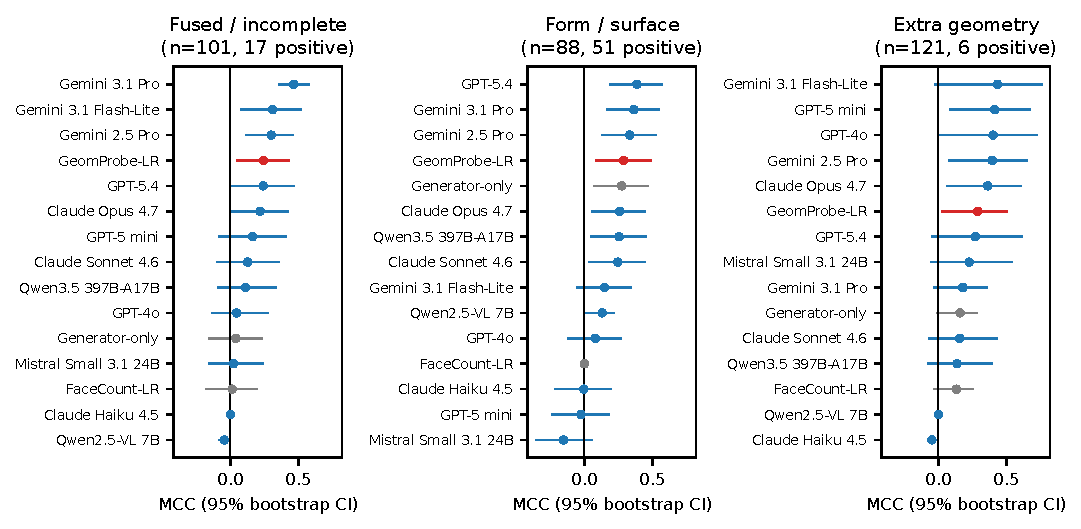
\includegraphics[width=\linewidth]{figures/fig2_forest_mcc.pdf}
  \caption{MCC on the three primary expert-agreement defects, with 95\% asset-bootstrap intervals. GeomProbe-LR is red, the twelve released VLM judges are blue, and the face-count and generator-only controls are grey.}
  \label{fig:forest}
\end{figure}
% src: results/main_comparison_expert_agreement.csv; results/RESULTS_milestone1.md

The paired tests do not support a claim of superiority either way against the strong VLMs.
After false-discovery correction, two of the 36 primary McNemar tests were significant.
The probe was more accurate than Mistral Small 3.1 24B on form/surface (adjusted \(p = 0.044\); \(\Delta\)MCC \(= 0.441\), 95\% CI [0.164, 0.725]).
The probe was less accurate than GPT-4o on extra geometry (adjusted \(p = 0.044\)).
That second contrast is a poor summary of association: GPT-4o predicted one positive against six true positives and its MCC interval is [0.000, 0.722], while the probe predicted 22 positives and the MCC difference has interval \([-0.481, 0.409]\).
One \(\Delta\)MCC interval excludes zero in favour of a strong VLM: Gemini 3.1 Pro on fused/incomplete (\(\Delta\)MCC \(= -0.222\), \([-0.437, -0.014]\)), and the corresponding McNemar test does not (adjusted \(p = 0.960\)).
Intervals that exclude zero in favour of the probe are confined to weaker judges (Claude Haiku 4.5, Qwen2.5-VL 7B, GPT-5 mini and Mistral Small 3.1 24B) and to individual defects.
Against Gemini 2.5 Pro, Gemini 3.1 Pro, GPT-5.4 and Claude Opus 4.7, no primary contrast was significant.
The expert cells are underpowered for those comparisons, particularly extra geometry.
% src: results/paired_tests_probe_vs_vlm.csv; results/main_comparison_expert_agreement.csv; results/RESULTS_milestone1.md

The negative controls behaved as specified.
On missing parts, GeomProbe-LR has MCC 0.024 (\([-0.164, 0.229]\); AUROC 0.570).
Gemini 2.5 Pro reaches 0.430 on the same cells (\(\Delta\)MCC \(= -0.406\), \([-0.741, -0.033]\), adjusted \(p < 0.001\)).
On pose/placement, with two positives, the probe MCC is \(-0.047\).
Face count is a weak control (macro-3 MCC 0.048).
Generator identity is not.
On form/surface the generator-only MCC is 0.273, against 0.288 for the full probe, so that result is largely which of the two generators produced the mesh.
Within-generator probe AUROCs are 0.796 (model A, 32 positives out of 45) and 0.664 (model B, 19 out of 43) for form/surface, 0.786 and 0.597 for fused/incomplete, and 0.785 and 0.705 for extra geometry, the last of these with a single positive in model B.
% src: results/main_comparison_expert_agreement.csv; results/paired_tests_probe_vs_vlm.csv; results/within_generator_auroc.csv; results/RESULTS_milestone1.md

Crowd labels were a poor teacher for form/surface.
Silver out-of-fold AUROC is 0.521 (MCC 0.068) for that defect, against 0.710 on the expert cells, and 0.704 / 0.686 (MCC 0.363 / 0.225) for fused/incomplete and extra geometry.
Classic manifold checks are nearly vacuous on this release: 98.4\% of the 678 GLBs are watertight, none have a non-manifold edge, and 0.4\% have a winding error.
The signals that vary are thin walls, genus, dihedral roughness, self-intersection (47\% of meshes) and hidden surface (49\% of meshes above 1\%), together with small components.
An exploratory scan of single features, selected on the expert cells and therefore optimistic, finds thin-wall fraction at 0.005 with AUROC 0.849 for form/surface and 0.778 for fused/incomplete, and small-component count with AUROC 0.770 for extra geometry.
Thirty-three feature--defect pairs pass a false-discovery threshold of 0.05.
The same ``messiness'' features predict several defect names, so they are not type-specific.
On the secondary target that marks a positive whenever either expert did, over all 129 assets, GeomProbe-LR has MCC 0.424, 0.153 and 0.270 for the three primary defects (AUROC 0.735, 0.640, 0.710).
Generator-only remains comparable on form/surface under that target (MCC 0.154).
% src: results/RESULTS_milestone1.md; results/ablations/expert_trained_on_silver.csv; results/exploratory_feature_auroc.csv; results/secondary_union_target_probes.csv

Figure~\ref{fig:gallery} shows eight meshes chosen by fixed rules, not by visual appeal: the highest probe probability among expert fused/incomplete and extra-geometry positives, the highest fused probability among assets that experts unanimously called free of all three primary defects, the lowest probability among expert form/surface positives, a bottom-decile MATE-3D geometry rating with a large thin-wall fraction, a top-decile rating with a high frozen defect score, and the clean GSO scans with the largest self-intersection and hidden-surface fractions.
The false positive and the high-MOS false alarm are part of the argument, not exceptions tucked out of the figure.
% src: figures/gallery_cases.csv

\begin{figure}[t]
  \centering
  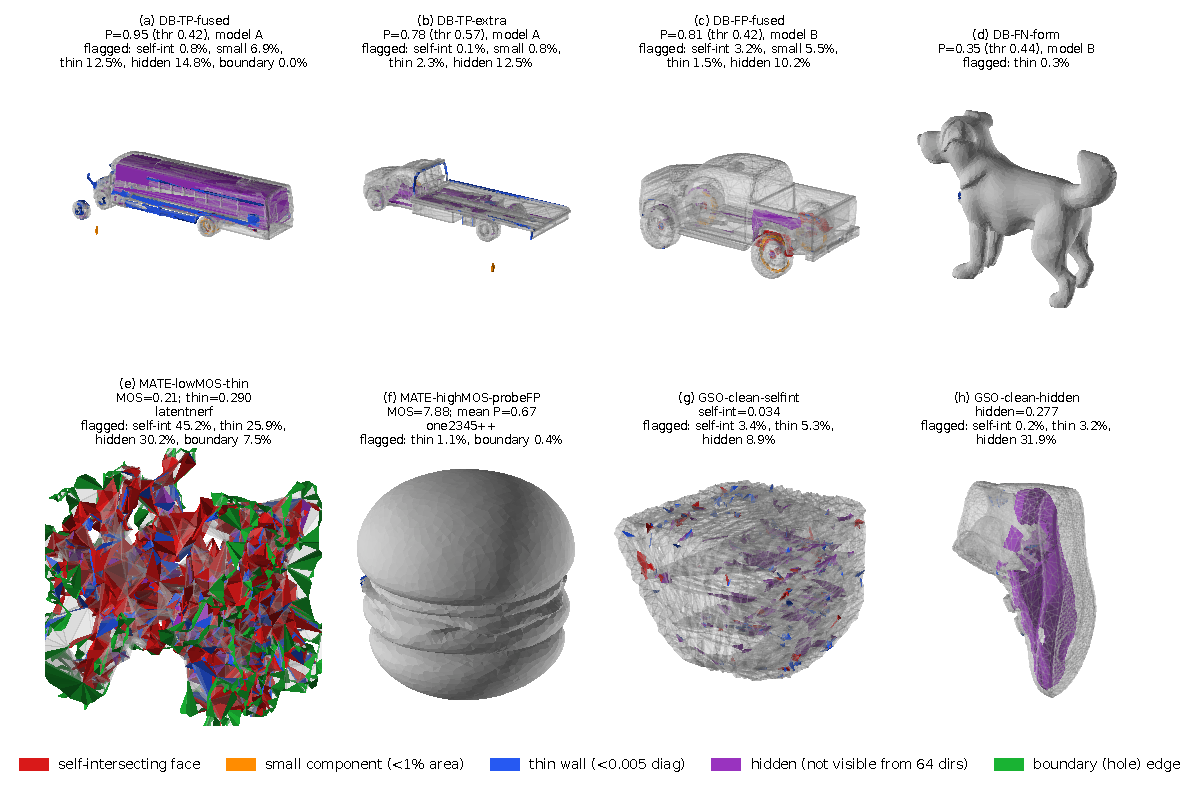
\includegraphics[width=\linewidth]{figures/fig1b_gallery.pdf}
  \caption{Cases selected by fixed rules. (a)~Expert fused/incomplete true positive, probe probability 0.95 against threshold 0.42, model A. (b)~Expert extra-geometry true positive, probability 0.78 against 0.57, model A. (c)~False positive: experts unanimous for no primary defect, fused probability 0.81, model B. (d)~Expert form/surface false negative, probability 0.35 against 0.44, model B. (e)~MATE-3D bottom-decile geometry MOS 0.21 with thin-wall fraction 0.290 (Latent-NeRF). (f)~MATE-3D top-decile MOS 7.88 with mean frozen defect probability 0.67 (One-2-3-45++). (g,h)~Clean GSO scans that already trigger self-intersection (face fraction 0.034) and hidden surface (0.277). Red: self-intersecting face. Orange: small component. Blue: thin wall. Purple: hidden surface. Green: boundary edge. Hidden-heavy meshes are drawn semi-transparent. 3D-DefectBench renders are shown under CC BY-NC 4.0 for non-commercial research.}
  \label{fig:gallery}
\end{figure}
% src: figures/gallery_cases.csv

\subsection{MATE-3D}
\label{sec:mate}

Table~\ref{tab:mate} and Figure~\ref{fig:mate} report the four estimands on the decimated meshes.
Three raw geometric checks replicate under the pre-registered rule.
Within generator, the thin-wall fraction at 0.005 has Spearman \(\rho = -0.195\) (95\% CI \([-0.255, -0.132]\), adjusted \(p = 0.001\)), the genus proxy has \(\rho = -0.110\) (\([-0.165, -0.055]\), adjusted \(p = 0.001\)), and the self-intersection fraction has \(\rho = -0.094\) (\([-0.144, -0.041]\), adjusted \(p = 0.003\)).
The frozen extra-geometry probability (\(\rho = -0.073\), \([-0.132, -0.012]\), adjusted \(p = 0.018\)) and the mean of the three frozen defect probabilities (\(\rho = -0.081\), \([-0.134, -0.027]\), adjusted \(p = 0.010\)) also replicate.
Every one of these within-generator correlations has absolute value at most 0.2.
They are detectable in 1{,}280 meshes and they are small.
% src: results/mate3d/mate3d_dec10k_correlations.csv; results/RESULTS_milestone2.md

\begin{table}[t]
  \centering
  \caption{MATE-3D geometry MOS, decimated meshes (\(n = 1{,}280\)). \(A\) is the pooled Spearman correlation. \(B\) is the within-generator Spearman correlation (primary), with a prompt-cluster interval. \(q\) is the Benjamini--Hochberg value over the nine primary predictors. \(C\) is mean within-prompt Kendall \(\tau\)-b. \(D\) residualises generator and prompt. The predicted sign is negative.}
  \label{tab:mate}
  \resizebox{\linewidth}{!}{%
  \begin{tabular}{lrrrrrl}
    \toprule
    Predictor & \(A\) & \(B\) [95\% CI] & \(q\) & \(C\) & \(D\) & Verdict \\
    \midrule
    Thin fraction (0.005) & $-0.181$ & $-0.195$ [$-0.255$, $-0.132$] & 0.001 & $-0.114$ & $-0.144$ & replicates \\
    Genus proxy & $-0.322$ & $-0.110$ [$-0.165$, $-0.055$] & 0.001 & $-0.263$ & $-0.118$ & replicates \\
    Self-intersection fraction & $-0.291$ & $-0.094$ [$-0.144$, $-0.041$] & 0.003 & $-0.245$ & $-0.057$ & replicates \\
    Dihedral mean & $-0.293$ & $-0.041$ [$-0.103$, $0.020$] & 0.191 & $-0.241$ & $-0.052$ & partial \\
    Hidden-surface fraction & $-0.297$ & $+0.028$ [$-0.033$, $0.088$] & 0.318 & $-0.257$ & $-0.041$ & partial \\
    \(P\)(form/surface) & $+0.150$ & $-0.046$ [$-0.108$, $0.018$] & 0.161 & $+0.120$ & $-0.052$ & fails \\
    \(P\)(fused/incomplete) & $-0.052$ & $-0.035$ [$-0.092$, $0.023$] & 0.234 & $-0.060$ & $-0.042$ & partial \\
    \(P\)(extra geometry) & $-0.218$ & $-0.073$ [$-0.132$, $-0.012$] & 0.018 & $-0.181$ & $-0.094$ & replicates \\
    Mean defect score & $+0.011$ & $-0.081$ [$-0.134$, $-0.027$] & 0.010 & $0.000$ & $-0.114$ & replicates \\
    \bottomrule
  \end{tabular}}
\end{table}
% src: results/mate3d/mate3d_dec10k_correlations.csv; results/RESULTS_milestone2.md

\begin{figure}[t]
  \centering
  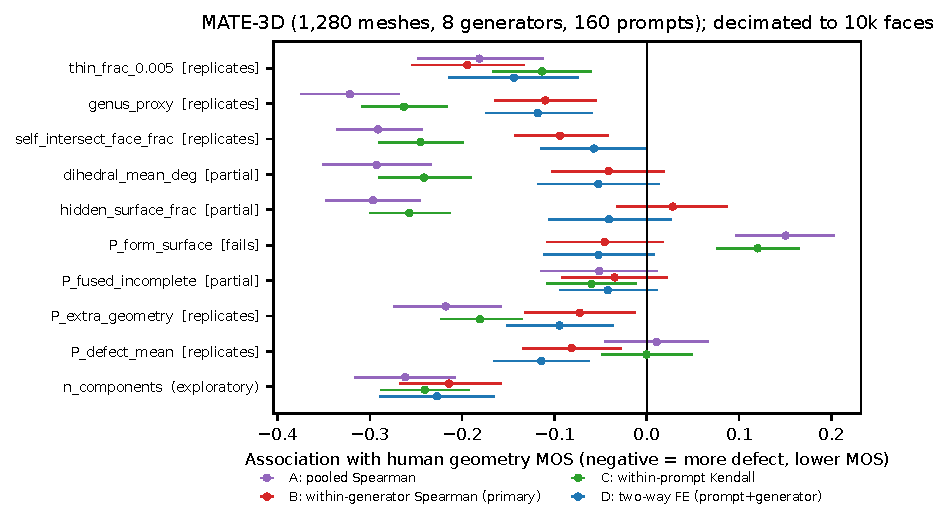
\includegraphics[width=\linewidth]{figures/fig5_mate3d_estimands.pdf}
  \caption{MATE-3D estimands for the nine primary predictors and, as an exploratory addition, component count. \(A\) pools all meshes. \(B\) is within generator and is the pre-registered primary. \(C\) is within prompt. \(D\) removes generator and prompt means. Negative values mean that a larger probe score accompanies a lower human geometry rating.}
  \label{fig:mate}
\end{figure}
% src: results/mate3d/mate3d_dec10k_correlations.csv; results/RESULTS_milestone2.md

Dihedral roughness and hidden surface are the cautionary rows.
Both have pooled correlations near \(-0.29\), and both lose that association once the generator is held fixed (dihedral \(\rho = -0.041\), interval including 0; hidden \(\rho = +0.028\)).
Across the eight generator means the same two features still look strongly related to mean MOS (descriptive Spearman \(-0.833\) and \(-0.762\), \(n = 8\)).
Generators that are rough or internally hidden are rated worse as generators.
Inside a generator, those two measurements do not track the rating.
The frozen form/surface probability fails outright: its pooled correlation is positive (\(+0.150\)), which is the wrong sign for a defect score.
The frozen fused/incomplete probability is only partial (\(\rho = -0.035\), interval including 0).
% src: results/mate3d/mate3d_dec10k_correlations.csv; results/RESULTS_milestone2.md

Figure~\ref{fig:heatmap} shows that the within-generator effects are not shared evenly.
The thin-wall correlation is \(-0.479\) for Latent-NeRF, \(-0.406\) for One-2-3-45++ and \(-0.313\) for SJC, and \(+0.073\) for Magic3D.
Dihedral mean is \(-0.431\) for One-2-3-45++ and \(-0.352\) for Latent-NeRF, and \(+0.257\) for both DreamFusion and TextMesh.
Hidden surface is \(+0.308\) for SJC.
A probe that is averaged over generators will describe a mixture of these regimes.
% src: results/mate3d/mate3d_dec10k_per_generator.csv; results/RESULTS_milestone2.md

\begin{figure}[t]
  \centering
  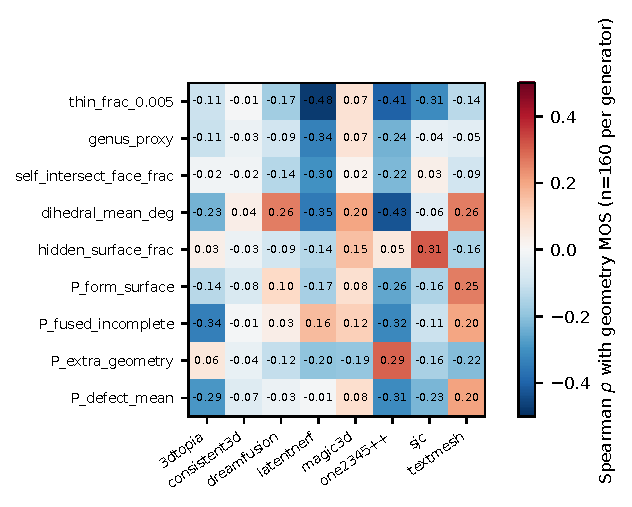
\includegraphics[width=\linewidth]{figures/fig6_mate3d_per_generator.pdf}
  \caption{Per-generator Spearman correlation between each pre-registered predictor and human geometry MOS on MATE-3D. Each column has 160 prompts. The sign is not stable across generators.}
  \label{fig:heatmap}
\end{figure}
% src: results/mate3d/mate3d_dec10k_per_generator.csv

Exploratory component features, which were not in the primary family of nine, have slightly larger within-generator correlations: component count \(\rho = -0.214\), large-component count \(\rho = -0.199\), and largest-component area fraction \(\rho = +0.192\), all with adjusted \(p < 0.001\) under the exploratory correction.
We do not promote them to a confirmed finding on the strength of this one corpus.
The undecimated meshes support the same verdicts for thin walls (\(-0.178\)), genus (\(-0.109\)), self-intersection (\(-0.063\)) and the mean defect score (\(-0.211\)).
Dihedral mean and hidden surface again fail within generator.
The form/surface probability again fails.
The fused/incomplete probability replicates only weakly (\(-0.060\), adjusted \(p = 0.048\)).
Decimation did not create the pattern.
% src: results/mate3d/mate3d_dec10k_correlations.csv; results/mate3d/mate3d_raw_correlations.csv; results/RESULTS_milestone2.md

\subsection{Injected defects on real scans}
\label{sec:gso}

Table~\ref{tab:gso} and Figure~\ref{fig:gsosev} give detection against the 120 clean decimated scans.
Holes and floaters are separated from the clean meshes with AUROC 1.000 at every severity, by boundary-edge fraction and by small-component count respectively.
At a threshold of zero both checks have sensitivity 1.00 and specificity 1.00: the clean decimated scans simply do not contain those signals, and every injected mesh does.
Self-intersection detects interpenetrating parts at AUROC 0.971, 0.978 and 0.986 and crossing sheets at 0.940, 0.965 and 0.977.
Hidden surface detects internal shells at 0.811, 0.869 and 0.912 and interpenetration at 0.835, 0.897 and 0.937.
Noise is visible in the dihedral mean at 0.753, 0.971 and 0.999.
Thin fins at S2 and S3 reach AUROC 0.952 on the 0.005 thin-wall fraction.
The S1 fin, which is thicker than that threshold, is at 0.651; the 0.010 thin-wall fraction reaches AUROC 0.826 on the same S1 fins.
Figure~\ref{fig:gsoex} shows one object, the alphabetically first scan for which all 22 variants probed successfully, at S3.
% src: results/gso/gso_detection.csv; results/RESULTS_milestone2.md; figures/gso_example_object.json

\begin{table}[t]
  \centering
  \caption{GSO injection. AUROC of the pre-registered target check against 120 clean meshes. Sensitivity and specificity are at a strict threshold of zero and are constant across severities for these checks. The S1 fin is thicker than 0.005 by design.}
  \label{tab:gso}
  \small
  \begin{tabular}{llcccc}
    \toprule
    Injected defect & Target check & S1 & S2 & S3 & Sens./spec.\ at 0 \\
    \midrule
    Holes & Boundary-edge fraction & 1.000 & 1.000 & 1.000 & 1.00 / 1.00 \\
    Floaters & Small-component count & 1.000 & 1.000 & 1.000 & 1.00 / 1.00 \\
    Interpenetrating part & Self-intersection & 0.971 & 0.978 & 0.986 & 1.00 / 0.79 \\
    Interpenetrating part & Hidden surface & 0.835 & 0.897 & 0.937 & 1.00 / 0.58 \\
    Crossing sheet & Self-intersection & 0.940 & 0.965 & 0.977 & 1.00 / 0.79 \\
    Hidden shell & Hidden surface & 0.811 & 0.869 & 0.912 & 1.00 / 0.58 \\
    Thin fin & Thin fraction (0.005) & 0.651 & 0.952 & 0.952 & 0.98--1.00 / 0.27 \\
    Noise & Dihedral mean & 0.753 & 0.971 & 0.999 & n/a \\
    \bottomrule
  \end{tabular}
\end{table}
% src: results/gso/gso_detection.csv; results/RESULTS_milestone2.md

\begin{figure}[t]
  \centering
  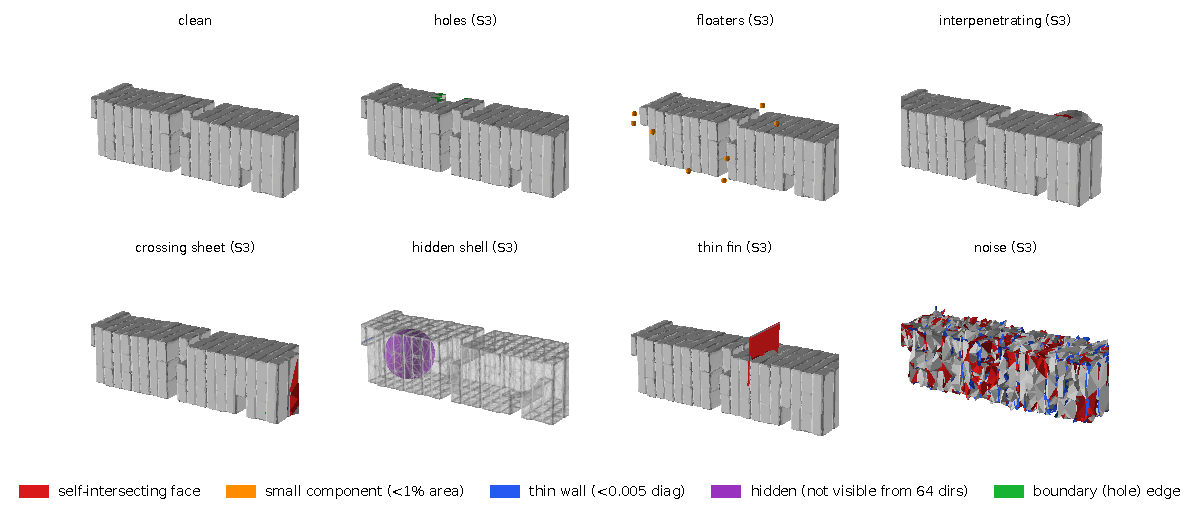
\includegraphics[width=\linewidth]{figures/fig3a_gso_examples.pdf}
  \caption{Clean decimated scan and the seven injected defects at severity S3 for one GSO object (alphabetically first with all 22 variants probed). The operators are applied to the real scan; they are not generator failures.}
  \label{fig:gsoex}
\end{figure}
% src: figures/gso_example_object.json; results/RESULTS_milestone2.md

\begin{figure}[t]
  \centering
  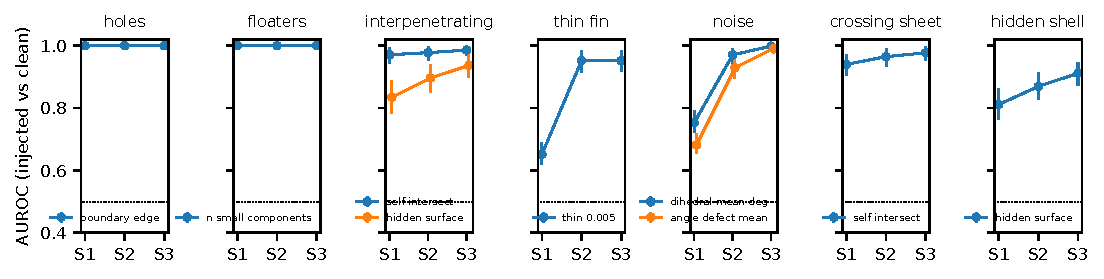
\includegraphics[width=\linewidth]{figures/fig3_gso_severity.pdf}
  \caption{AUROC of each pre-registered target check as injection severity increases from S1 to S3. Holes and floaters are saturated at S1. The thin-fin curve uses the 0.005 threshold, which is below the S1 plate thickness.}
  \label{fig:gsosev}
\end{figure}
% src: results/gso/gso_detection.csv

Specificity at zero is the first place validity and ``clean'' diverge.
Of the clean decimated scans, 21\% already self-intersect, 42\% have hidden-surface fraction above zero, and 73\% have thin-wall fraction above zero, so the strict self-intersection, hidden-surface and thin-wall checks have specificities 0.79, 0.58 and 0.27.
A zero threshold is a property of the decimated scan, not a certificate that a rater would call the mesh clean.

The calibrated thresholds move the operating point to the other extreme.
On the 200 crowd-labelled defect-free 3D-DefectBench assets, the 95th percentile is 0.044 of faces self-intersecting, hidden-surface fraction 0.128, 3.05 small components, thin-wall fraction 0.050, and genus proxy 48.1.
Sensitivity at this \(\tau_c\) is at most 0.10 for the self-intersection targets, at most 0.32 for the hidden-surface targets, and 0 for one and for three floaters (the ten-floater severity does cross 3.05).
Figure~\ref{fig:ecdf} plots the two reference distributions.
Generated assets that the crowd called defect-free sit far to the right of the clean scans.
A gate set on human ``defect-free'' labels will pass meshes that a strict geometric definition rejects, and a strict gate will reject meshes that raters accept.
% src: results/gso/tau_calibrated.json; results/gso/gso_detection.csv; results/RESULTS_milestone2.md

\begin{figure}[t]
  \centering
  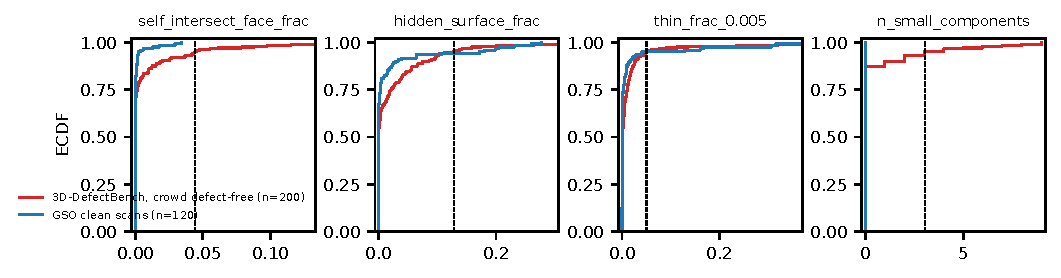
\includegraphics[width=\linewidth]{figures/fig7_ecdf_clean_reference.pdf}
  \caption{Empirical distributions of four checks on crowd-labelled defect-free 3D-DefectBench assets (\(n = 200\)) and on clean decimated GSO scans (\(n = 120\)). Dashed lines are the calibrated thresholds \(\tau_c\), the 95th percentile of the crowd-labelled defect-free set.}
  \label{fig:ecdf}
\end{figure}
% src: results/gso/tau_calibrated.json; results/RESULTS_milestone2.md

The checks are sensitive and, except for holes and floaters, not type-specific.
Figure~\ref{fig:cross} is the S2 cross-talk matrix.
At S3, hidden-surface fraction responds to interpenetration (AUROC 0.94), crossing sheets (0.89), noise (0.86) and thin fins (0.89), not only to hidden shells (0.91).
Self-intersection responds to noise (1.00) and to fins (0.96) as well as to the two operators aimed at it.
Boundary fraction and small-component count stay near chance off their own targets, with one mechanical exception: a crossing sheet also creates a boundary, so boundary fraction detects it at AUROC 1.000.
% src: results/gso/gso_crosstalk_auroc.csv; results/RESULTS_milestone2.md

\begin{figure}[t]
  \centering
  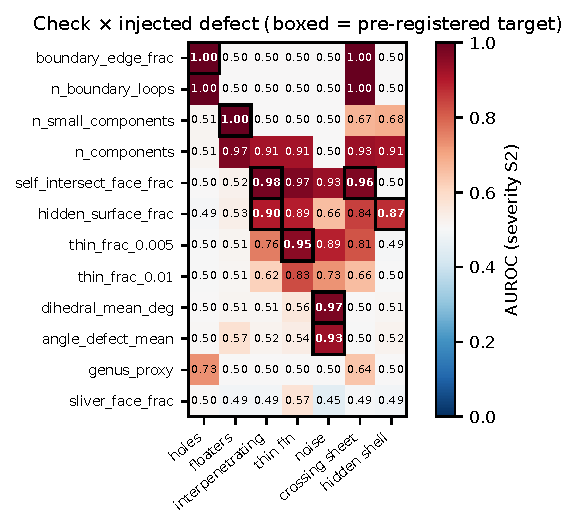
\includegraphics[width=\linewidth]{figures/fig4_gso_crosstalk.pdf}
  \caption{AUROC of each check (rows) against each injected defect at severity S2 (columns). Boxed cells are the pre-registered targets. Off-target cells near 1 show cross-talk; cells near 0.5 show that the check did not move.}
  \label{fig:cross}
\end{figure}
% src: results/gso/gso_crosstalk_auroc.csv

\subsection{Ablations and fusion}
\label{sec:ablate}

Family-only models, trained on the silver holdout and scored on the expert-agreement cells, put most of the expert-set AUROC in the topology family.
Topology alone (six features) reaches AUROC 0.801, 0.770 and 0.786 on fused/incomplete, form/surface and extra geometry (MCC 0.395, 0.572, 0.188), at or above the full 30-feature model (AUROC 0.695, 0.710, 0.742).
Boundary and manifold features alone sit near chance (AUROC 0.564, 0.533, 0.573), which matches the watertightness of this benchmark.
Leave-one-family-out changes AUROC by at most about 0.06.
MCC is less stable than AUROC, because the silver out-of-fold threshold is fragile: dropping self-intersection or triangle quality from the form/surface model pushes that threshold to 1.0 and the expert MCC to 0.
Single-feature rules chosen after seeing the expert set---and therefore optimistic---give genus AUROC 0.763, hidden surface 0.755 and self-intersection 0.698 for fused/incomplete; thin walls 0.849 and dihedral mean 0.691 for form/surface; and small-component count 0.770 for extra geometry.
Choosing the topology-only model because it won on the expert cells would be test-set selection.
We report it as an ablation.
The pre-registered model remains the 30-feature regression.
Figure~\ref{fig:ablate} summarises the family AUROCs.
% src: results/ablations/lofo_family_rules.csv; results/RESULTS_milestone2.md

\begin{figure}[t]
  \centering
  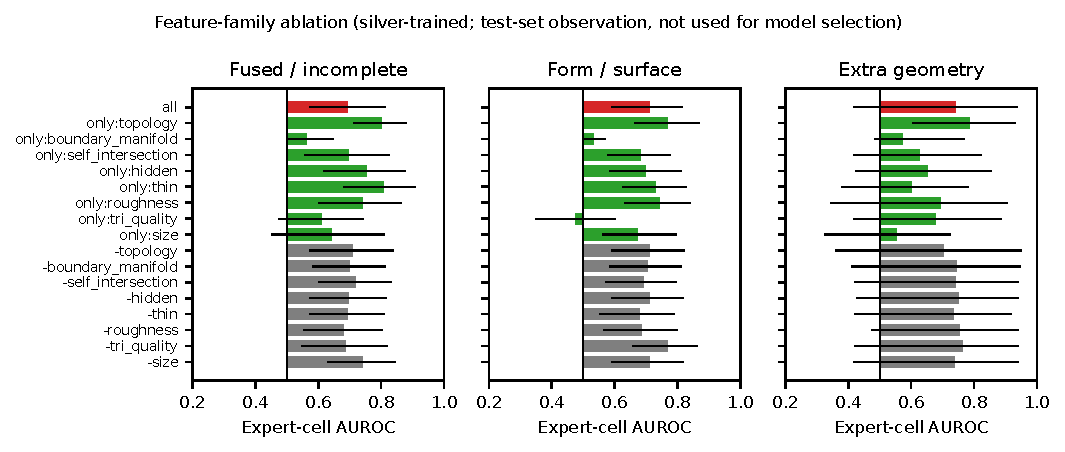
\includegraphics[width=\linewidth]{figures/fig8_ablation_families.pdf}
  \caption{Family-only and leave-one-family-out AUROC on the expert-agreement cells, for models trained on the silver holdout. Topology alone matches or exceeds the full model. That comparison was not used to select the reported predictor.}
  \label{fig:ablate}
\end{figure}
% src: results/ablations/lofo_family_rules.csv

Training on the expert cells does not beat training on the noisy silver labels.
Across 50 repeats of five-fold cross-validation on the agreement cells, expert-trained AUROC is 0.719 against 0.695 for the frozen silver model on fused/incomplete (mean difference \(+0.024\), positive in 68\% of repeats), 0.729 against 0.710 on form/surface (\(+0.019\), 72\% of repeats), and 0.502 against 0.742 on extra geometry (\(-0.240\), positive in 0\% of repeats; six positives).
A model fit on all expert cells and applied to the silver holdout has AUROC 0.599, 0.563 and 0.467, against silver out-of-fold AUROC 0.704, 0.521 and 0.686.
Eighty-eight to 121 expert cells did not outperform 548 crowd labels.
% src: results/RESULTS_milestone2.md; results/ablations/expert_trained_on_silver.csv

Learned fusion does not improve the strong VLMs.
A logistic regression on the frozen probe logit plus the VLM vote, evaluated by 50 repeats of five-fold cross-validation on the expert cells, has mean \(\Delta\)MCC across the 12 VLMs of \(-0.008\) (fused/incomplete), \(+0.107\) (form/surface) and \(0.000\) (extra geometry).
For the four strong VLMs from the paired analysis---Gemini 2.5 Pro, Gemini 3.1 Pro, GPT-5.4 and Claude Opus 4.7---the mean differences are \(-0.060\), \(-0.014\) and \(-0.021\).
An earlier fusion fit on the silver holdout and applied once to the expert cells helps weaker VLMs (mean \(\Delta\)MCC \(+0.08\) on fused/incomplete and \(+0.11\) on extra geometry) and does not help the best one: Gemini 3.1 Pro on fused/incomplete moves from 0.463 to 0.416.
% src: results/RESULTS_milestone2.md; results/ablations/fusion_repeated_cv.csv; results/exploratory_fusion.csv

The training-free AND rule---flag the defect only if the VLM and the frozen probe both do---is the most consistent combination we tried, and it is still a weak result.
\(\Delta\)MCC is positive in 29 of 36 VLM--defect pairs, negative in 4 and zero in 3.
Averaged over those four VLMs, MCC moves from 0.305 to 0.354 on fused/incomplete, from 0.334 to 0.366 on form/surface, and from 0.301 to 0.518 on extra geometry.
After false-discovery correction, 1 of the 36 AND comparisons is significant: Mistral Small 3.1 24B on fused/incomplete (\(\Delta\)MCC \(= 0.168\), [0.063, 0.297]).
The best VLM does not gain on the defect it already wins.
Gemini 3.1 Pro on fused/incomplete moves from 0.463 to 0.450 (\(\Delta\)MCC \(= -0.014\), \([-0.222, 0.182]\)).
The OR rule can move the other way: for that same cell, OR lowers MCC by 0.129 (\([-0.195, -0.072]\); no bootstrap resample out of 10{,}000 had a non-negative difference, so the adjusted value is below \(10^{-3}\)).
Figure~\ref{fig:and} plots the AND differences.
Directionally consistent, underpowered, and not a reason to replace a strong judge.
% src: results/RESULTS_milestone2.md; results/ablations/and_or_rule_bootstrap.csv

\begin{figure}[t]
  \centering
  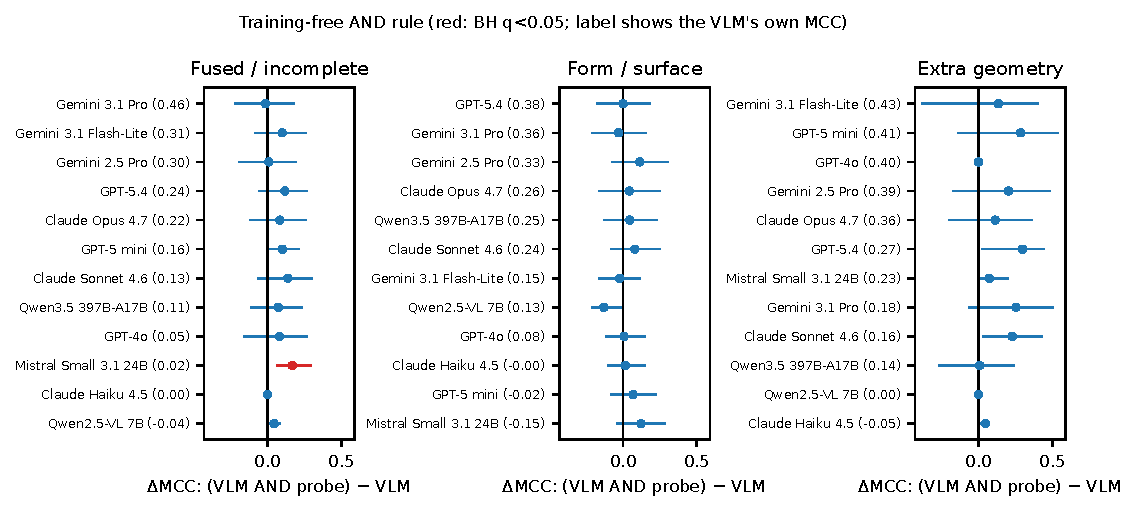
\includegraphics[width=\linewidth]{figures/fig9_and_rule.pdf}
  \caption{Change in MCC when a released VLM vote is conjoined with the frozen probe flag (AND), on the three primary expert-agreement defects. Intervals are bootstrap intervals. One of the 36 comparisons remains significant after Benjamini--Hochberg correction.}
  \label{fig:and}
\end{figure}
% src: results/ablations/and_or_rule_bootstrap.csv; results/RESULTS_milestone2.md

\subsection{Hi3DBench}
\label{sec:hi3d}

Hi3DBench was pre-registered as a secondary, within-generator scale-up.
Its object-level scores are pseudo-labels from the Hi3DEval M$^{2}$AP multi-agent MLLM pipeline, not human ratings \citep{zhang2025hi3deval}.
The primary target, \texttt{geometry\_score}, is Geometry Plausibility.
The secondary target, \texttt{geo\_detail\_score}, is geometric detail.
The four predictors were thin-wall fraction at 0.005, genus proxy, self-intersection fraction and component count, each with a negative predicted sign, on SPAR3D, TRELLIS, TripoSR, InstantMesh, Hunyuan3D and CRM \citep{huang2025spar3d,xiang2025trellis,tochilkin2024triposr,xu2024instantmesh,zhao2025hunyuan3d2,wang2024crm}.
Unique3D was excluded for time and disk budget before scoring \citep{wu2024unique3d}.
We analysed 2{,}797 labelled meshes from 510 image prompts.
Meeting the replication rule here means agreement with that automated judge.
% src: analysis/PREREGISTRATION_M3_hi3dbench.md; results/RESULTS_milestone3.md; results/hi3dbench/hi3dbench_meta.json

All four predictors meet the rule on Geometry Plausibility (Table~\ref{tab:hi3d}, Figure~\ref{fig:hi3d}).
Within generator, thin-wall fraction has Spearman \(\rho = -0.111\) (95\% CI \([-0.157, -0.066]\), adjusted \(p < 0.001\)), genus proxy has \(\rho = -0.063\) (\([-0.106, -0.018]\), adjusted \(p = 0.001\)), self-intersection fraction has \(\rho = -0.042\) (\([-0.084, -0.001]\), adjusted \(p = 0.026\)) and component count has \(\rho = -0.066\) (\([-0.108, -0.025]\), adjusted \(p = 0.001\)).
Every within-generator correlation has absolute value at most 0.111.
The effects are small.
The direction matches the MATE-3D within-generator signs for thin walls, genus and self-intersection, at a smaller magnitude, and it is not a human replication.
% src: results/hi3dbench/hi3dbench_correlations.csv; results/RESULTS_milestone3.md

\begin{table}[t]
  \centering
  \caption{Hi3DBench Geometry Plausibility, an MLLM pseudo-label (\(n = 2{,}797\)). Secondary evidence. \(A\) is the pooled Spearman correlation. \(B\) is the within-generator Spearman correlation (primary), with a prompt-cluster interval. \(q\) is the Benjamini--Hochberg value over the four predictors. \(C\) is mean within-prompt Kendall \(\tau\)-b. \(D\) residualises generator and prompt (2{,}000 bootstrap resamples; the other intervals use 10{,}000). The predicted sign is negative. ``Replicates (B only)'' means \(B\) meets the rule while \(D\) is significantly positive.}
  \label{tab:hi3d}
  \resizebox{\linewidth}{!}{%
  \begin{tabular}{lrrrrrl}
    \toprule
    Predictor & \(A\) & \(B\) [95\% CI] & \(q\) & \(C\) & \(D\) & Verdict \\
    \midrule
    Thin fraction (0.005) & $+0.009$ & $-0.111$ [$-0.157$, $-0.066$] & $<0.001$ & $+0.085$ & $-0.023$ & replicates \\
    Genus proxy & $-0.028$ & $-0.063$ [$-0.106$, $-0.018$] & 0.001 & $+0.033$ & $+0.005$ & replicates \\
    Self-intersection fraction & $+0.022$ & $-0.042$ [$-0.084$, $-0.001$] & 0.026 & $+0.074$ & $+0.044$ & replicates (B only) \\
    Component count & $-0.220$ & $-0.066$ [$-0.108$, $-0.025$] & 0.001 & $-0.175$ & $-0.006$ & replicates \\
    \bottomrule
  \end{tabular}}
\end{table}
% src: results/hi3dbench/hi3dbench_correlations.csv; results/RESULTS_milestone3.md; results/hi3dbench/hi3dbench_meta.json

The within-generator result is not robust to prompt adjustment.
The two-way estimand \(D\) is about zero for thin walls (\(-0.023\), \([-0.067, 0.022]\)), genus (\(+0.005\), \([-0.035, 0.046]\)) and component count (\(-0.006\), \([-0.046, 0.034]\)).
For self-intersection it is positive (\(+0.044\), \([0.005, 0.083]\)), so the interval excludes zero in the direction opposite the prediction.
Between generators the sign flips for thin walls and self-intersection.
Within a prompt, the generator whose mesh has more thin walls, or more self-intersection, tends to receive a higher Geometry Plausibility score (\(C = +0.085\), \([0.051, 0.119]\), and \(C = +0.074\), \([0.034, 0.114]\)).
TRELLIS has by far the highest mean thin-wall fraction (0.185, against at most 0.058 for the other five generators) and the second-highest mean Geometry Plausibility (5.863).
Component count, which the Geometry Plausibility criterion names in connection with floating parts, has the largest pooled and within-prompt associations (\(A = -0.220\), \(C = -0.175\)) and only \(-0.066\) within generator.
% src: results/hi3dbench/hi3dbench_correlations.csv; results/hi3dbench/hi3dbench_per_generator.csv; results/hi3dbench/hi3dbench_meta.json; results/RESULTS_milestone3.md

The per-generator correlations are heterogeneous (Figure~\ref{fig:hi3d}).
They are strongest for CRM, from \(-0.221\) to \(-0.312\) across the four predictors (\(n = 247\)), and for InstantMesh on thin walls (\(-0.214\)) and genus (\(-0.170\)).
They are weaker for Hunyuan3D, SPAR3D and TRELLIS (absolute values at most 0.092).
A single pooled number describes a mixture of these regimes.
% src: results/hi3dbench/hi3dbench_per_generator.csv; results/RESULTS_milestone3.md

\begin{figure}[t]
  \centering
  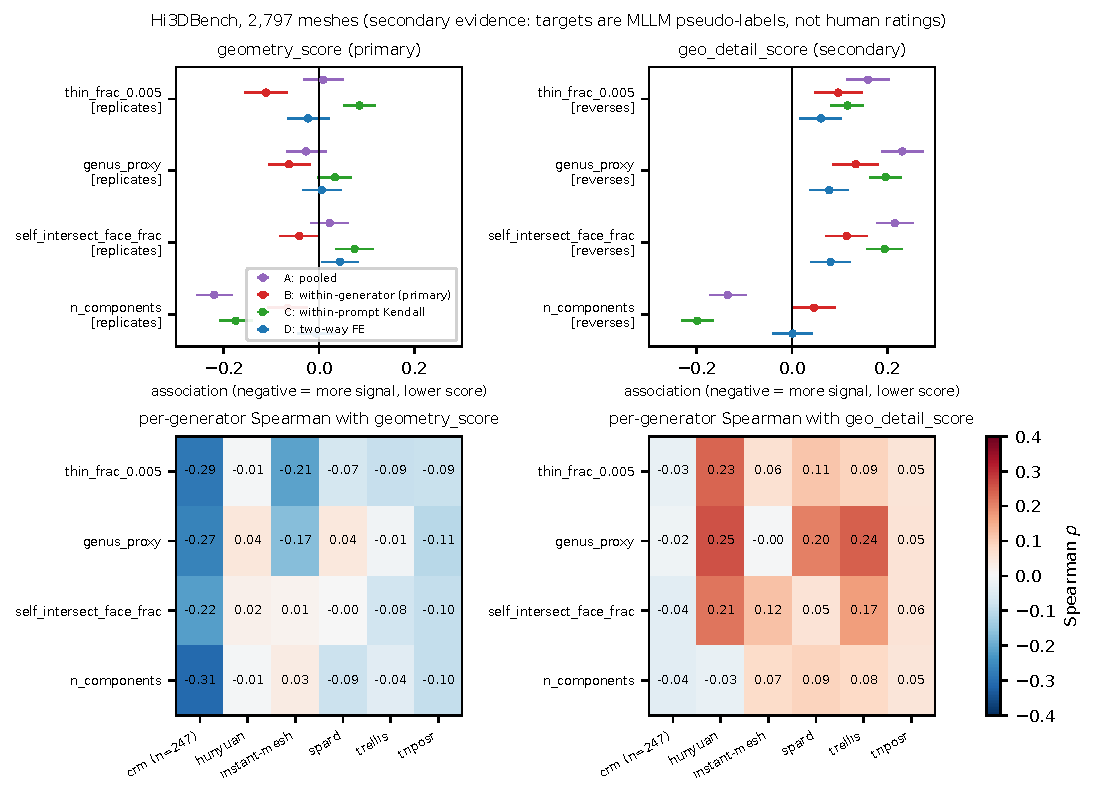
\includegraphics[width=\linewidth]{figures/fig10_hi3dbench.pdf}
  \caption{Hi3DBench, 2{,}797 labelled meshes. Top: estimands \(A\)--\(D\) with prompt-cluster intervals for Geometry Plausibility (primary pseudo-label) and geometric detail (secondary pseudo-label). Bottom: per-generator Spearman correlations. Negative values mean that a larger probe score accompanies a lower pseudo-label. These targets are MLLM outputs, not human ratings.}
  \label{fig:hi3d}
\end{figure}
% src: results/hi3dbench/hi3dbench_correlations.csv; results/hi3dbench/hi3dbench_per_generator.csv; results/RESULTS_milestone3.md

The geometric-detail score reverses all four within-generator signs.
Thin walls, genus, self-intersection and component count have \(\rho = +0.097\) (\([0.047, 0.147]\)), \(+0.134\) (\([0.086, 0.180]\)), \(+0.115\) (\([0.071, 0.158]\)) and \(+0.046\) (\([0.001, 0.092]\)), with adjusted \(p\)-values at most 0.016.
The pooled correlations are \(+0.159\), \(+0.231\), \(+0.216\) and \(-0.135\).
The same ``defect'' signals co-occur with geometric detail as judged by the MLLM pipeline.
That is a complexity confound: a validity gate that penalises thin walls, genus or self-intersection will also penalise meshes this automated judge calls detailed.
% src: results/hi3dbench/hi3dbench_correlations.csv; results/RESULTS_milestone3.md

\section{Discussion}
\label{sec:disc}

\subsection{What the probes measure}
The injection study is the cleanest evidence the probes do what their definitions say.
On real scans, a hole becomes a boundary and a disconnected icosphere becomes a small component, with AUROC 1.000 at the smallest severity we tried, and with perfect specificity at a zero threshold.
% src: results/gso/gso_detection.csv; results/RESULTS_milestone2.md
Self-intersection, hidden surface, thin walls and dihedral roughness then pick up the operators aimed at them once the operator is large enough to move the corresponding scalar.
That is geometric validity in the narrow sense: a named, local, mesh-theoretic failure, inserted into geometry that was not generated to fool a judge.

The same study limits how far a scalar can be read as a defect type.
At high severity, self-intersection also rises under noise and under thin fins, and hidden surface rises under interpenetration, crossing sheets, noise and fins.
A gate can reject a mesh for ``this quantity exceeded a threshold''.
It cannot, without further rules, file the failure under the benchmark's noun for it.
Holes and floaters are the exceptions.
Their checks stayed specific.

Two operating points should be reported, because they answer different questions.
A threshold of zero asks whether the signal is absent.
On these decimated scans it is absent for boundaries and small components, and it is often present for self-intersection, hidden surface and thin walls.
A mesh can be a careful scan of a physical object and still fail a strict thin-wall or self-intersection check after decimation.
The calibrated thresholds ask a different question: what level of the same signal is still typical of generated assets that crowd workers called free of geometric defects?
Those levels are high---several percent of faces self-intersecting or hidden, several small components, a genus proxy in the tens---and they are high enough that the injected defects often fall below them.
Human ``defect-free'' is not geometric cleanliness.
Figure~\ref{fig:gallery} is the same fact on single meshes: an expert-unanimous clean asset can score like a defect, a high geometry MOS can score like a defect, and a clean scan can light up the hidden-surface and self-intersection checks.

\subsection{What they do not measure}
Perceived quality, within a generator, is only weakly related to these scalars.
The within-generator correlations that replicated on MATE-3D are negative, as predicted, and none of the nine pre-registered ones exceeds 0.2 in absolute value.
% src: results/RESULTS_milestone2.md; results/mate3d/mate3d_dec10k_correlations.csv
Dihedral roughness and hidden surface look associated with geometry MOS in the pooled table and in the eight generator means, and they are not associated with it inside a generator.
The form/surface classifier has the same structure on 3D-DefectBench: generator identity alone reaches MCC 0.273, next to the probe's 0.288, and the silver crowd labels for that defect were close to chance (out-of-fold AUROC 0.521).
% src: results/main_comparison_expert_agreement.csv; results/ablations/expert_trained_on_silver.csv; results/RESULTS_milestone1.md
A feature that mostly distinguishes model A from model B will look like a defect detector if the two models have different defect rates.
The within-generator AUROCs are the ones that survive that reading, and they are uneven.

Hi3DBench points the same way, and only as secondary evidence.
The four pre-registered predictors meet the negative within-generator rule for Geometry Plausibility, with absolute correlations at most 0.111, and the two-way fixed-effect estimand is about zero or, for self-intersection, positive.
Within a prompt, more thin walls or more self-intersection accompanies a higher score from the same automated judge.
The geometric-detail score then reverses all four within-generator signs.
A validity gate that penalises thin walls, genus or self-intersection will also penalise meshes that this MLLM pipeline calls detailed.
Agreement with that pipeline is not human validation.
% src: results/RESULTS_milestone3.md; results/hi3dbench/hi3dbench_correlations.csv

Prompt-conditioned defects are outside the probes' scope, and the negative controls say so.
Missing parts and pose depend on the text.
The probe is near null; the VLMs are not.
A validity gate that fails an asset for a missing part it cannot see is the wrong tool, just as a VLM vote is the wrong tool for certifying that a mesh has no self-intersection.

The expert-set horse-race should be read at the width of its intervals.
Macro MCC 0.158 over five defects is 8th of 15 predictors.
% src: results/macro_mcc.csv; results/RESULTS_milestone1.md
Macro MCC 0.272 over the three primary defects sits below Gemini 2.5 Pro and Gemini 3.1 Pro (0.341 and 0.335).
The comparisons against those models, and against GPT-5.4 and Claude Opus 4.7, were not significant.
Some of that is power: extra geometry has six agreed positives, and McNemar scores accuracy, so a balanced probe that predicts 22 positives is punished relative to a VLM that predicts one.
We do not describe the probe as better than a VLM judge.
``Comparable to mid-tier VLM judges'' is as far as these cells support.
% src: results/macro_mcc.csv; results/paired_tests_probe_vs_vlm.csv; results/main_comparison_expert_agreement.csv; results/RESULTS_milestone1.md

Fusion does not change that recommendation.
Learning a weight on the probe logit and the VLM vote did not help the four strongest models.
The training-free AND rule moved MCC up in 29 of 36 pairs and survived correction in one pair, a weak VLM on one defect.
% src: results/RESULTS_milestone2.md; results/ablations/and_or_rule_bootstrap.csv
The OR rule significantly hurt Gemini 3.1 Pro on fused/incomplete.
An extra-geometry mean that jumps under AND is not, with six positives and no surviving corrected test, evidence of a reliable gain.
Conjunctions remain a hypothesis for a larger expert set.

The topology-only ablation is easy to over-read.
On the expert cells, six topology features match or beat the full model.
That comparison uses the same cells that would be flattered by any family we noticed after the fact, and the pre-registered single-feature shortlist was already chosen after seeing those cells.
The external tests of the underlying quantities are the MATE-3D correlations and the GSO detections, not the ablation ranking.
We would not ship a topology-only model on the basis of this test set.

\subsection{Recommendations for evaluators}
\begin{enumerate}
  \item Report geometric validity beside perceptual scores, not inside them.
  A leaderboard that sorts generators by VLM votes or by geometry MOS is answering a perceptual question.
  Holes, floaters, self-intersection, hidden shells and thin walls can be columns of their own, with the definition and the threshold written down.
  \item Publish the continuous score and at least two operating points: a strict zero threshold, and any threshold derived from human-accepted meshes.
  State which reference set produced the threshold.
  A pass at the crowd-calibrated \(\tau_c\) of this paper is not evidence that the mesh is geometrically clean, and a failure at zero is not evidence that a rater would reject a scan.
  \item Include a generator-only baseline and a within-generator estimand whenever a geometric feature is correlated with a human or VLM score.
  For genus, self-intersection, roughness and hidden surface, the pooled MATE-3D correlation is larger in magnitude than the within-generator correlation, and for roughness and hidden surface the within-generator interval includes zero.
  \item Use the probes as a gate and as a diagnostic, and keep a perceptual or VLM judge for preference, prompt fidelity and defects that are defined by the prompt.
  If the two are combined, pre-register the rule, freeze the probe threshold on a separate split, and correct for the number of judges tested.
  The AND results here are directionally consistent and mostly non-significant.
  \item Do not select the feature family on the evaluation split.
  If a simpler topology model is preferable, confirm it on a later corpus.
  The single-feature AUROCs in Section~\ref{sec:db} are exploratory.
  \item Name the label. Expert votes, crowd votes and MLLM pseudo-labels are different targets.
  The Hi3DBench analysis is agreement with the Hi3DEval automated judge.
  It is not a second human validation.
  Do not treat a negative association with Geometry Plausibility as a licence to penalise thin walls, genus or self-intersection without a separate check on detail: on the geometric-detail pseudo-label those three signals reverse.
  \item Expect cross-talk when turning a score into a defect name.
  Boundary fraction and small-component count were specific under our operators.
  Self-intersection and hidden surface were not.
  A repair router that trusts one scalar as a type label will send noise and thin fins to the wrong fixer.
\end{enumerate}
% src: results/RESULTS_milestone1.md; results/RESULTS_milestone2.md; results/RESULTS_milestone3.md; results/macro_mcc.csv; results/mate3d/mate3d_dec10k_correlations.csv; results/gso/gso_detection.csv; results/gso/tau_calibrated.json; results/hi3dbench/hi3dbench_correlations.csv

\section{Limitations}
\label{sec:limit}

The expert-agreement cells are small, and they are a selected subset of the expert split: both annotators agreed.
Extra geometry has six positives, pose/placement has two, and the paired tests against strong VLMs were underpowered.
We therefore treat non-significance as absence of evidence.
A larger expert set could move the mid-pack MCC in either direction.
The secondary union target, which scores all 129 expert assets, is more prevalent and is not paired with VLM votes, because those votes were not released for disagreement cells.

3D-DefectBench contains two generators.
The form/surface result is entangled with that binary identity, which is why the generator-only control and the within-generator AUROCs are part of the primary report rather than a footnote.
Crowd labels, especially for form/surface, were a weak training signal.
Fitting the same regression on the expert cells did not fix this: there are not enough agreed labels, and extra geometry got worse.

The VLM side is one released configuration, not a new sweep of views, prompts or renderers.
3D-DefectBench already studied that sensitivity; we used the published votes so that the comparison would cost no API calls and would match the authors' MCCs.
We did not measure whether a different VLM pipeline would agree more or less with the probes.
Binary VLM AUROC is balanced accuracy.
MCC is the comparison that does not depend on that choice.

The injections are simpler than generator failures.
Each operator adds one kind of damage to a scanned household object, on a mesh that has already been welded and decimated.
Generated meshes are dirty in several of these ways at once, which is what the cross-talk matrix and the calibrated thresholds describe, and they are not a sample of GSO.
Clean-scan specificity will not transfer to a corpus in which every mesh is a generator output.
Conversely, AUROC against clean scans is an easier detection task than ranking two generated meshes.
Decimation can change thickness and intersection counts.
The undecimated MATE-3D run is the check we have, and it did not change the verdicts; we did not repeat the injection study without decimation.

Ray probes depend on a fixed sample of 20{,}000 points and on Embree, and self-intersection depends on PyMeshLab.
We verified that installing the system libraries PyMeshLab needs did not change probe outputs, but we do not claim bit-identity across library versions we did not run.
The classifier is linear and was not tuned.
A more flexible model might fit the silver labels more tightly; the silver form/surface labels look too noisy for that to be the binding constraint, and we did not test it.

Hi3DBench is secondary evidence only.

Its labels are MLLM pseudo-labels from the Hi3DEval M$^{2}$AP pipeline, not human ratings.
The within-generator correlations with Geometry Plausibility have absolute value at most 0.111.
They are heterogeneous across generators and not robust once prompt and generator means are removed.
Unique3D was excluded before scoring.
The reversal on the geometric-detail score means a validity gate fitted to Geometry Plausibility can punish complexity.
% src: results/RESULTS_milestone3.md; results/hi3dbench/hi3dbench_correlations.csv; analysis/PREREGISTRATION_M3_hi3dbench.md

DB-3DME could not be probed because the release we used contains renders rather than meshes.
3DGen-Bench was left out because the files are gated.
Texture, material and prompt alignment are out of scope for a geometry-only probe.
The work is a single-author, CPU-only study on public data.
% src: results/RESULTS_milestone1.md; results/RESULTS_milestone2.md; results/RESULTS_milestone3.md; analysis/PREREGISTRATION.md; analysis/PREREGISTRATION_M3_hi3dbench.md


\section{Conclusion}
\label{sec:conc}

Deterministic probes measured the geometric failures we inserted into real scans, and they did not measure perceived quality.
Holes and floaters were detected perfectly at every severity we tried.
Self-intersection, hidden shells, thin walls and noise were detected once they were large enough to move the matching scalar, with cross-talk that prevents those scalars from being used as defect names.
On expert labels from 3D-DefectBench the same probes, read out by a logistic regression trained only on crowd votes, landed in the middle of a field of VLM judges and did not significantly differ from the strongest of them.
On MATE-3D the associations with human geometry ratings that survive a within-generator analysis are small, and some associations that look large in a pooled table are generator identity.
A secondary comparison with Hi3DBench pseudo-labels shows the same weak within-generator direction (absolute correlation at most 0.111) and a reversal on geometric detail, which is a complexity confound for a validity gate rather than a human replication.
% src: results/RESULTS_milestone3.md; results/hi3dbench/hi3dbench_correlations.csv
Thresholds taken from generated assets that people called clean are loose enough to miss injected defects, while strict thresholds already fire on clean scans.
Evaluators can use these probes as a validity gate and as a control that makes generator confounds visible.
Perceptual and VLM judges remain necessary for the question the probes do not answer.

\section*{Resources and data availability}
The probe implementation, the injection and analysis code, and the per-asset probe statistics can be released with this paper.
3D-DefectBench meshes are not redistributed: the dataset is CC BY-NC 4.0 and was used for non-commercial research only \citep{zhao2026defectbench}.
MATE-3D and Google Scanned Objects are CC BY 4.0 \citep{zhang2025mate3d,downs2022gso}.
Hi3DBench is distributed under the MIT licence on its dataset card \citep{zhang2025hi3deval}.
DB-3DME, as released, provided GIF renders rather than meshes \citep{jia2026db3dme}.
The author works on modelfy.art (\url{https://modelfy.art}), an online image- and text-to-3D service; no modelfy.art models, assets or data were used in this study.

\section*{Declaration of competing interest}
The author is affiliated with modelfy.art, a commercial 3D-generation service, which could benefit from improved evaluation of generated 3D assets.
The study uses only public datasets and open-source tools; no modelfy.art system was evaluated.

\section*{Acknowledgements}
We thank the authors of 3D-DefectBench, MATE-3D, Hi3DBench, DB-3DME and Google Scanned Objects for releasing data, labels and, in the case of 3D-DefectBench, VLM predictions.
Probe code uses Trimesh, PyMeshLab and Embree \citep{trimesh,cignoni2008meshlab,wald2014embree}.


\appendix
\section{Probe definitions and configuration}
\label{app:probes}

Table~\ref{tab:config} records the constants that were frozen before expert-set scoring.
Lengths are fractions of the bounding-box diagonal after normalisation.
The genus feature passed to the classifier is \(\log(1+g)\) with \(g\) as in Equation~\eqref{eq:genus}.
Every other non-negative feature is passed through \(\log(1+x)\) and then standardised on the training split.
Standardisation, class weights and the decision threshold are part of the frozen predictor, not of the mesh probes.
The probes themselves have no fitted parameters.
Sampling uses seed 0.

\begin{table}[t]
  \centering
  \caption{Frozen probe and classifier configuration.}
  \label{tab:config}
  \small
  \begin{tabular}{lp{8.6cm}}
    \toprule
    Item & Value \\
    \midrule
    Vertex welding & round to \(10^{-6}\), replace by the group mean \\
    Small component & area below 1\% of the total surface \\
    Surface samples & 20{,}000, area-weighted, seed 0 \\
    Visibility directions & 64, Fibonacci sphere \\
    Ray offset & \(10^{-4}\) \\
    Thin-wall tolerances & 0.005 and 0.010 \\
    Sliver & triangle quality \(q < 0.1\) \\
    Dihedral exceedances & \(30^\circ\), \(60^\circ\), \(90^\circ\), length-weighted \\
    Decimation & quadric edge collapse to 10{,}000 faces; preserve topology, boundary and normals; planar quadrics \\
    Classifier & L2 logistic regression, \(C = 1\), balanced class weights, at most 5{,}000 iterations \\
    Threshold & MCC-optimal on 5-fold stratified out-of-fold scores, seed 0 \\
    Training assets & 548 silver-holdout meshes; asset 609 excluded \\
    \bottomrule
  \end{tabular}
\end{table}
% src: geomcheck/probes.py; analysis/PREREGISTRATION.md; results/RESULTS_milestone1.md

The primary decision thresholds locked by that rule, and then applied unchanged to every later corpus, are 0.416 for fused/incomplete, 0.440 for form/surface and 0.574 for extra geometry.
% src: results/ablations/lofo_family_rules.csv

Injection severities, in order S1, S2, S3, are: hole area fraction 0.002, 0.010, 0.040 across three patches; 1, 3 or 10 floaters of radius 0.01, offset by 0.05 along the normal; ellipsoid major radius 0.05, 0.10, 0.20 with transverse radii at half the major radius; fin thickness 0.008, 0.004, 0.002 on a plate of extent \(0.2 \times 0.2\); normal noise of standard deviation 0.001, 0.003, 0.010; duplicated patch area fraction 0.005, 0.020, 0.050 rotated by \(30^\circ\); hidden-shell radius 0.25, 0.50, 0.90 times the distance from the chosen interior point (the farthest from the surface among 20{,}000 uniform candidates) to the surface.
The per-object seed is the SHA-256 of the object name, reduced modulo \(2^{32}\).
The subset of 120 scans was drawn with \texttt{random.Random(0)} from the 1{,}033 Fuel models.
% src: scripts/gso_inject.py; analysis/PREREGISTRATION_M2.md

Feature families used in the ablation are those fixed in the milestone-2 plan: topology (component count, largest-component area fraction, small-component count and area, large-component count, genus proxy); boundary and manifold (boundary-edge fraction and length, boundary loops, winding inconsistency, duplicate-face fraction); self-intersection (face and area fractions); hidden surface; thin walls (defined-thickness fraction, both thin fractions, median thickness); roughness (dihedral mean and three exceedances, both angle-defect summaries); triangle quality (median, 5th percentile, both sliver fractions, edge-length coefficient of variation); size (face count).
% src: analysis/PREREGISTRATION_M2.md

\section{Pre-registration record and deviations}
\label{app:prereg}

\subsection{What was locked, and when}
The milestone-1 plan (expert-set comparison on 3D-DefectBench) was committed as git revision 024f7eb on 2026-09-27 at 16:22 UTC+8, before any expert-set probe score was used for evaluation.
The recorded SHA-256 prefix of that plan is 42280714.
It fixes the silver-holdout training split, the exclusion of asset 609, the 30-feature logistic regression, the face-count and generator-only controls, the three primary defects, the two negative controls, the 10{,}000-resample asset bootstrap with seed 12345, and Benjamini--Hochberg control over the 36 primary McNemar tests.
The milestone-2 plan was committed as 78d6623 at 16:44 UTC+8, before MATE-3D scoring, GSO injection and the ablations.
It fixes the four MATE-3D estimands, the nine primary predictors and their negative sign, the replication rule, the seven injection operators and their target checks, the two GSO operating points, the object bootstrap with seed 2028, and the family ablations.
The milestone-3 plan was committed as c003104 at 17:36 UTC+8, before Hi3DBench scoring.
It fixes a secondary analysis of MLLM pseudo-labels, the four predictors named in Section~\ref{sec:hi3d}, and the decision to skip Unique3D for time and disk budget.
The milestone-3 analysis script was committed as b528343, also before scoring.
Frozen milestone-1 models were refit only as a reproducibility check; the refit reproduces the milestone-1 thresholds.
% src: analysis/PREREGISTRATION.md; analysis/PREREGISTRATION_M2.md; analysis/PREREGISTRATION_M3_hi3dbench.md; results/RESULTS_milestone1.md; results/RESULTS_milestone3.md

\subsection{What had already been seen}
Before the milestone-1 plan we had read the released VLM prediction files, in order to check that our MCC code matches the benchmark authors to three decimal places on all 12 models, and we had counted label prevalences.
Probe outputs on 11 expert GLBs were inspected as an engineering smoke test, without labels and without a score against labels.
Before the milestone-2 plan we had seen the head and tail of the MATE-3D ratings table while checking its format, and probe values on the eight meshes of the prompt ``A blue vase'' while testing decimation.
No correlation between a probe and a rating had been computed, and no injection had been run.
A further engineering smoke test, one MATE-3D prompt and one GSO object, was run to confirm that the pipeline executed.
It was not used to choose features, thresholds or severities.
% src: analysis/PREREGISTRATION.md; analysis/PREREGISTRATION_M2.md

\subsection{Deviations and disclosures}
The first decimator we tried, \texttt{fast\_simplification}, was rejected before scoring because it broke topology and introduced holes on the blue-vase meshes.
It was replaced by the PyMeshLab topology-preserving collapse described in Section~\ref{sec:method}.
That choice is a preprocessing deviation from an earlier engineering attempt, and it was made before any confirmatory statistic.
System OpenGL libraries were installed during the project so that PyMeshLab would load.
Probe outputs were compared before and after that installation and were bit-identical.
Asset 609 remained excluded.
Unique3D remained excluded from the Hi3DBench plan, before scoring.
No \(C\), no feature list and no threshold was changed after the expert set, the MATE-3D ratings, the injection outcomes or the Hi3DBench scores were computed.

Two analyses are easier to mistake for confirmatory than they are.
The single-feature rules for genus, hidden surface, self-intersection, thin walls, dihedral mean and small components were named after the milestone-1 expert AUROCs, and the milestone-2 plan says so.
Their expert-set numbers are optimistic; the pre-registered external checks are MATE-3D and GSO.
The topology-only model outscoring the full model is a result on the expert cells.
It was not used to replace GeomProbe-LR.
Hi3DBench labels are disclosed in the milestone-3 plan as MLLM pseudo-labels.
They are not a deviation from a human protocol, because no human protocol was registered for that corpus.
The scores are reported in Section~\ref{sec:hi3d}.
They are secondary agreement with an automated judge, not a human validation, and the small within-generator correlations are not a null finding.
% src: analysis/PREREGISTRATION_M2.md; analysis/PREREGISTRATION_M3_hi3dbench.md; results/RESULTS_milestone2.md; results/RESULTS_milestone3.md


\bibliographystyle{unsrtnat}
\emergencystretch=2em
\bibliography{refs}

\end{document}
